%Plantilla basada en "Template for Masters / Doctoral Thesis" (plantilla disponible en writeLaTex) que subió LaTeXTemplates.com

\documentclass[12pt]{book}
\usepackage[paperwidth=17cm, paperheight=22.5cm, bottom=2.5cm, right=2.5cm]{geometry}
\usepackage{fixltx2e}
\usepackage{amssymb,amsmath,amsthm} %paquete para símbolo matemáticos
\usepackage[spanish]{babel}
\usepackage[utf8]{inputenc} %Paquete para escribir acentos y otros símbolos directamente
\usepackage{enumerate}
\usepackage{graphicx}
\usepackage{float}
\usepackage{multirow}
\usepackage{chicago}
\usepackage[nottoc]{tocbibind}
\usepackage[hyphens]{url}
\usepackage[pdftex,
            pdfauthor={Emiliano Kokic},
            pdftitle={Reconocimiento semi-supervisado de entidades nombradas mediante redes convolucionales en escalera},
            pdfsubject={Licenciatura en Ciencias de la Computación}]{hyperref}

\usepackage[colorinlistoftodos]{todonotes}

\begin{document}

%----------------------------------------------------------------------------------------
%	COMANDOS PERSONALIZADOS
%----------------------------------------------------------------------------------------

%SI TU TESIS TIENE TEOREMAS Y DEMOSTRACIONES, PUEDES DESCOMENTAR Y USAR LOS SIGUIENTES COMANDOS

%\renewcommand{\proofname}{Demostración}
%\providecommand{\norm}[1]{\lVert#1\rVert} %Provee el comando para producir una norma.
%\providecommand{\innp}[1]{\langle#1\rangle} 
%\newcommand{\seno}{\mathrm{sen}}
%\newcommand{\diff}{\mathrm{d}}

%\newtheorem{teo}{Teorema}[section] 
%\newtheorem{cor}[teo]{Corolario}
%\newtheorem{lem}[teo]{Lema}

%\theoremstyle{definition}
%\newtheorem{dfn}[teo]{Definición}

%\theoremstyle{remark}
%\newtheorem{obs}[teo]{Observación}

%\allowdisplaybreaks


%----------------------------------------------------------------------------------------
%	PORTADA
%----------------------------------------------------------------------------------------

\title{Reconocimiento semi-supervisado de entidades nombradas mediante redes convolucionales en escalera}

\begin{titlepage}
\begin{center}

\textsc{\Large{Facultad de Matemática, Astronomía, Física y Computación}}\\[1em]
\textsc{\large{Universidad Nacional de Córdoba}}\\[0.5em]

\begin{figure}[h]
\begin{center}

\includegraphics[width=.3\linewidth]{images/unc.jpg}
\end{center}
\end{figure}
\vspace{-0.1em}

\LARGE{\textbf{Reconocimiento semi-supervisado de entidades nombradas mediante redes convolucionales en escalera}}\\[0.5em]

\textsc{\normalsize{Tesis para obtener el título de}}\\

\textsc{\large{Licenciado en Ciencias de la Computación}}\\

\textsc{\normalsize{Autor:} \Large{Emiliano Kokic}}\\

\textsc{\normalsize{Director:} \large{Cristian Cardellino}}

\end{center}

\vspace*{\fill}
\textsc{Córdoba, Argentina \hspace*{\fill} 2019}

\end{titlepage}


%----------------------------------------------------------------------------------------
%	DEDICATORIA
%----------------------------------------------------------------------------------------

% \pagestyle{empty}
% \frontmatter

% \chapter*{}
% \begin{flushright}
% \textit{DEDICATORIA}
% \end{flushright}


%----------------------------------------------------------------------------------------
%	AGRADECIMIENTOS
%----------------------------------------------------------------------------------------

% \chapter*{Agradecimientos}
% %\markboth{AGRADECIMIENTOS23}{AGRADECIMIENTOS} % encabezado 

% ¡Muchas gracias a todos!


%----------------------------------------------------------------------------------------
%	PREFACIO
%----------------------------------------------------------------------------------------

\chapter*{Resumen}

\pagestyle{plain}
\markboth{PREFACIO23}{PREFACIO} % encabezado 

El presente trabajo de tesis consiste en la exploración de un método de aprendizaje automático semi-supervisado llamado Redes Convolucionales en Escalera. La problemática que se decide abordar para la evaluación de dicho modelo es el Reconocimiento de Entidades Nombradas, una tarea muy relevante dentro del área de Procesamiento del Lenguaje Natural. Para realizar el estudio fue indispensable contar con WiNER, un corpus anotado de Wikipedia de gran calidad y fácil acceso. A su vez se estudian alternativas de representación de las palabras de acuerdo a su contexto. Se utiliza el bien conocido modelo Word2Vec para la generación de \textit{embeddings} de palabras junto con la aplicación de estrategias que los combinan. En particular, resulta que el uso de capas convolucionales es una gran herramienta para la extracción de atributos del contexto. Se implementaron distintas arquitecturas de modelos, cada una de ellas con su versión supervisada (a modo de baseline) y semi-supervisada (al agregar las redes en escalera). Cada arquitectura tiene distintos tipos de instancias de entrenamiento, en algunos casos utilizando el etiquetado de palabras así como también el etiquetado de secuencias. Finalmente, luego de definir las métricas de evaluación se realizaron los experimentos pertinentes encontrando el modelo de Redes Convolucionales en Amplitud en Escalera como el más prometedor. Si bien los resultados obtenidos no son del estado del arte en cuanto a la tarea de reconocimiento de entidades nombradas, se visualiza que los modelos semi-supervisados de redes neuronales en escalera generalizan mejor y su performance no disminuye en gran medida al de los supervisados gracias al uso complementario de datos no anotados.

\vspace{10mm}

The present work consists in the exploration of a semi-supervised machine learning method called Convolutional Ladder Networks. A very relevant task within the Natural Language Processing area is the Named-entity recognition, this is the problem that is decided to deal for the model evaluation. In order to carry out this study, it was essential to have WiNER, an annotated corpus of Wikipedia of great quality and easy access. At the same time, alternative strategies for the word representations according to their context are studied. The well-known Word2Vec model is used to generate word embeddings along with the application of strategies that combine them. In particular, it turns out that the use of convolutional layers is a great tool for context features extraction. Different model architectures were implemented, each of them with their supervised version (as a baseline) and the semi-supervised one (when adding ladder networks). Each architecture has different types of training instances, in some cases using word tagging as well as sequence tagging. Finally, once the experiments were executed, we found the Wide Convolutional Ladder Networks model as the most promising. Although the results obtained are not from the state of the art in terms of the task of recognizing named entities, it is found that semi-supervised models of ladder neural networks generalize better and their performance does not decrease greatly to that of supervised ones thanks to the complementary use of unlabeled data.

%----------------------------------------------------------------------------------------
%	TABLA DE CONTENIDOS
%---------------------------------------------------------------------------------------

\tableofcontents


%----------------------------------------------------------------------------------------
%	TESIS
%----------------------------------------------------------------------------------------
\mainmatter %empieza la numeración de las páginas
\pagestyle{headings}

\chapter{Introducción y motivación}

\section{Introducción}

El \textbf{Aprendizaje Automático} (del inglés, \textit{Machine Learning}) es una rama de la inteligencia artificial que ha adoptado diferentes definiciones a lo largo de la historia. En particular, Tom M. Mitchell proporcionó una definición formal de los algoritmos estudiados en el campo del aprendizaje automático: ``Se dice que un programa de computadora aprende de la experiencia E con respecto a alguna clase de tareas \textit{T} y rendimiento \textit{P} si su desempeño en las tareas \textit{T}, medido por \textit{P}, mejora con experiencia \textit{E}.'' \cite{Mitchell:1997:ML:541177}.

El aprendizaje automático tiene una amplia gama de aplicaciones. Un problema típico que se puede abordar es la predicción de precios de inmuebles \footnote{\url{https://www.kaggle.com/c/house-prices-advanced-regression-techniques}}. A partir del uso de distintas características de inmuebles tales como sus metros cuadrados, cantidad de habitaciones, antigüedad, etc., y los precios asociados se genera un modelo, el cual a partir de nuevos datos de entrada (``características'' o ``atributos'' de un inmueble) proporciona como salida una estimación del precio del mismo.

% https://www.kaggle.com/erick5/predicting-house-prices-with-machine-learning
Los tipos de algoritmos de aprendizaje automático difieren de acuerdo a su enfoque, el tipo de datos que ingresan, o el que generan, y el tipo de tarea o problema que pretenden resolver.

Una de las tareas más comunes es el \textbf{aprendizaje supervisado}, el cual produce una función que establece una correspondencia entre los datos de entrada y los datos de salida (conocidos como ``etiquetas''). Dentro del aprendizaje supervisado nos encontramos con problemas de regresión (como el anterior ejemplo de predicción de precios de inmuebles) que tratan de etiquetar a los datos en un rango numérico (i.e. la etiqueta es continua), o 
con problemas de clasificación que trata de etiquetar a los datos en un conjunto finito de etiquetas discretas (o clases). Un ejemplo de clasificación es el reconocimiento facial de Facebook \footnote{\url{https://www.facebook.com/facialrecognitionapp/}} que utiliza para el auto-etiquetado de imágenes. La tarea concreta que el algoritmo debe realizar es, a partir de una imagen, detectar los rostros de personas que se encuentran en la misma y asociar a cada uno de ellos con el nombre de la persona correspondiente.

El \textbf{aprendizaje no supervisado} es otra tarea común en aprendizaje automático, donde todo el proceso de modelado se lleva a cabo sobre un conjunto de ejemplos formado tan sólo por datos que no tienen ninguna información sobre valor o categoría asociada (i.e. no tienen ``etiquetas''). El objetivo de una tarea de aprendizaje no supervisado generalmente está en el descubrimiento de patrones o señales que puedan explicar los datos. Un problema interesante que el aprendizaje no supervisado puede atacar es el modelado de temas en noticias, donde el objetivo es poder agrupar palabras o incluso oraciones que pertenezcan a una misma categoría. Este es un ejemplo de lo que en aprendizaje no supervisado se conoce como \textit{clustering} (a veces conocido en la literatura del español como ``agrupamiento'') donde la dificultad muchas veces se encuentra en saber elegir la cantidad de agrupaciones (\textit{clusters}) para posteriormente hacer un análisis de las mismas.

Finalmente, existe un híbrido de los métodos nombrados anteriormente llamado \textbf{aprendizaje semi-supervisado}. El análisis del habla es un ejemplo clásico del valor que pueden aportar este tipo de modelos\footnote{\url{https://medium.com/@jrodthoughts/understanding-semi-supervised-learning-a6437c070c87}}. Abordar esta tarea en particular, con un modelo netamente supervisado, requeriría de muchos recursos humanos que establezca manualmente cuáles son las salidas que debe tener el modelo para ciertos datos de entrada (proceso que se conoce como etiquetado). Esto se debe a que etiquetar audio no es trivial y es, precisamente, donde un modelo de aprendizaje semi-supervisado puede ser de gran ayuda al requerir pocos datos anotados y muchos no anotados. En este trabajo de tesis se estudia en detalle un modelo de aprendizaje semi-supervisado.

\section{Motivación}

El \textbf{procesamiento de lenguaje natural}, abreviado PLN o NLP (del inglés \textit{Natural Language Processing}), es un campo de las ciencias de la computación, la inteligencia artificial y la lingüística que estudia las interacciones con computadores mediante lenguaje humano. Se ocupa de la formulación e investigación de mecanismos eficaces computacionalmente para la comunicación entre personas y máquinas por medio de lenguajes naturales (e.g. español, inglés, etc). PLN es en sí mismo una de las tareas más complejas que estudia la inteligencia artificial, conociéndose como un problema AI-completo. PLN está, a su vez, dividido en diversas subáreas que buscan resolver distintos problemas de índole más específico, algunos estando más cerca de ser considerados ``resueltos''.

La extracción de información es una de las tareas de PLN que todavía requiere trabajo. Es además, una tarea fundamental en el análisis de texto libre para poder estructurar los datos que pueden obtenerse del texto de manera automática y poder así democratizar mejor el acceso a dicha información. 

Una de las tareas más importantes que se engloban dentro del área que de extracción de información es el \textbf{reconocimiento de entidades nombradas} \footnote{\url{https://en.wikipedia.org/wiki/Named-entity_recognition}}. Esta tarea busca ubicar y clasificar ciertas entidades de un texto no estructurado en categorías predefinidas, como  nombres de personas y organizaciones, ubicaciones, expresiones temporales, cantidades, valores monetarios, entre otras. Supongamos que tenemos la siguiente oración:

\vspace{2.5mm}

Jim bought 300 shares of Acme Corp. in 2006.

\vspace{2.5mm}

Potenciales entidades a reconocer serían las siguientes:

\vspace{2.5mm}

[Jim]$_{Person}$ bought 300 shares of [Acme Corp.]$_{Organization}$ in [2006]$_{Time}$

\vspace{5mm}

Como tantas otras áreas de trabajo en procesamiento de lenguaje natural, existen buenos recursos para realizar dicha tarea de manera automática en inglés. Sin embargo, muchas veces dependiendo del dominio y/o el idioma, la calidad de estos datos puede disminuir considerablemente. Es entonces que entra en escena las ventajas de trabajar con métodos semi-supervisados que aprovechen la enorme cantidad de datos no anotados que circulan libremente por Internet. El problema con los métodos semi-supervisados es que a veces se hace difícil evaluarlos y compararlos directamente sobre tareas que los aprovechen, puesto que dichas tareas no tienen punto de comparación. Se hace necesario entonces saber si dichos métodos son útiles en tareas ya establecidas.

El objetivo de esta tesis es la exploración de un método semi-supervisado conocido como ``redes neuronales convolucionales en escalera'' \cite{DBLP:journals/corr/RasmusVHBR15}. Este método es utilizado originalmente para procesamiento de imágenes, en esta tesis se adaptó a la tarea de reconocimiento de entidades nombradas. Como punto de comparación en dicha tarea, el trabajo se basa en el corpus WiNER \cite{WiNER-Ghaddar-Langlais}.

\section{Estructura de la tesis}

En el Capítulo \ref{chapter:chapter2} comenzamos analizando el trabajo de \cite{WiNER-Ghaddar-Langlais} sobre el corpus WiNER, generado a partir de la Wikipedia y seleccionado para nuestra investigación. Posteriormente se describe la problemática de representación de palabras de acuerdo al contexto en el que ocurren y estrategias que buscan resolver dicho problema a partir del trabajo de \cite{iacobacci-etal-2016-embeddings}. Finalmente hacemos una mención detallada de las redes neuronales en escalera propuestas en el trabajo de \cite{DBLP:journals/corr/RasmusVHBR15}, describiendo su arquitectura y particularidades. 

En el Capítulo \ref{chapter:chapter3} se realiza un análisis del corpus WiNER mencionando como fue procesado en base a distintas decisiones. Se introducen los distintos tipos de instancias de entrenamiento utilizadas en los modelos junto con una descripción de las métricas de evaluación seleccionadas. Por último, se detallan las arquitecturas de los modelos utilizados.

En el Capítulo \ref{chapter:chapter4} se identifican los distintos experimentos realizados junto con sus resultados e interpretaciones. 
En el Capítulo \ref{chapter:chapter5} se proporcionan las conclusiones de esta tesis junto con el trabajo futuro.

%\chapter{Análisis del problema}
%\include{chapters/problem_analysis}

\chapter{Trabajo relacionado} \label{chapter:chapter2}

\section{WiNER: Un corpus anotado de Wikipedia para Reconocimiento de Entidades Nombradas}

Como se mencionó previamente, en esta tesis se estudiará el impacto de una técnica de aprendizaje semi-supervisado, redes convolucionales en escalera, en una tarea de reconocimiento de entidades nombradas. Para eso se buscó un recurso de referencia que pudiera servirnos a la hora de establecer una base de experimentos en donde evaluar las redes en escalera.

Si bien hay varias opciones disponibles para estudiar, muchas de ellas eran pagas o bien requerían un proceso de registro que llevaba mucho tiempo. Es por eso que se decidió trabajar con la Wikipedia como base. Ahora bien, una opción sería hacer todo el trabajo de preproceso y diseñar el corpus de base para los experimentos. Sin embargo, eso también consume mucho tiempo.
 
Convertir Wikipedia en un corpus de entidades nombradas anotadas con tipos es una tarea que recibió cierta atención a lo largo de los últimos años. En particular, en el trabajo de \cite{WiNER-Ghaddar-Langlais} se propuso una nueva metodología aplicada a la Wikipedia en inglés para construir WiNER, un gran corpus anotado de alta calidad. 

Para realizar esto aplicaron un pipeline de anotación, el cual consta de tres etapas. En primera instancia se consideran los enlaces directos de cada artículo objetivo, buscando en su texto los títulos de los artículos que se acceden. A su vez, cuentan con un recurso previo\footnote{\url{http://rali.iro.umontreal.ca/rali/en/}} que enumera todas las menciones del texto que se refieren al concepto principal de un artículo. Esto posibilita realizar una relación entre las correferencias del recurso y los títulos accedidos. A cada una de estas coincidencias se le asigna una etiqueta con la entidad asociada proveniente de una tabla de correferencias. 

Con el fin de obtener una mayor cobertura, en una segunda etapa ya se consideran enlaces anidados, buscando en el artículo objetivo los títulos de los artículos alcanzados y en caso de haber coincidencias se les asignan las entidades nombradas correspondientes. Finalmente, estos títulos emparejados en la segunda etapa también se comparan con sus menciones en la tabla de correferencias.

En cuanto a la evaluación del corpus generado, por un lado se realiza una evaluación manual a partir de un subconjunto de 1000 menciones. En esta etapa se mide la exactitud (o \textit{accuracy} en inglés) obtenida luego de aplicar cada etapa del pipeline. 

Posteriormente, se utilizan otros corpus de entidades anotadas, entre ellos uno clásico de referencia, el CONLL-2003 obtenido en el trabajo de \cite{TjongKimSang:2003:ICS:1119176.1119195}. Se compara el desempeño de distintos modelos con la métrica F1-score sobre las clases para nombres de personas (PER), organizaciones (ORG) y lugares (LOC) donde lo que varía fijado un modelo es la proporción del corpus WiNER que se utiliza y el corpus de evaluación, siendo el modelo LSTM-CRF \cite{DBLP:journals/corr/HuangXY15} el más prometedor.

\section{Embeddings para desambiguación del sentido de palabras}

Uno de los problemas fundamentales a la hora de lidiar con algoritmos de aprendizaje automático es la manera de representar los datos. Esto se debe a que los algoritmos esperan como entrada un vector de números de tamaño fijo. E.g., las imágenes pueden representarse mediante la intensidad de cada uno de sus píxeles. 

En el caso del trabajo con texto, la representación de los datos es algo particularmente complejo. Principalmente se debe a la naturaleza discreta de las palabras, donde las representaciones clásicas suelen ser ralas (i.e. vectores de mucha dimensionalidad, pero con muchos ceros). 

Ejemplos de este tipo de representaciones son los vectores \textit{one-hot encodings}. Para estos casos cada vector tiene la dimensionalidad del total de palabras del vocabulario, donde cada palabra se corresponde con una componente del vector. Entonces cada palabra es representada por un vector de todos 0's salvo un 1 en la componente que tenga asociada. Dado que el tamaño del vocabulario en general es considerablemente grande provoca que estos vectores sean de gran dimensionalidad. Además, hay que notar que los vectores no preservan información sobre el contexto en el que sucedieron las palabras en el texto, sino que son representaciones discretas de las mismas.

Hace unos años comenzaron a utilizarse más las representaciones distribuidas de las palabras, donde cada palabra es representada por las palabras de su vecindad. En particular, aparecieron los \textit{word embeddings}, vectores densos y continuos que codifican la probabilidad de una palabra dada su vecindad. 

Existen diferentes métodos para obtener \text{word embeddings}, pero todos tienen el objetivo de generar representaciones de palabras a partir de un corpus sin etiquetas.

En particular, el algoritmo Word2Vec \cite{DBLP:journals/corr/MikolovSCCD13}, explora dos arquitecturas de modelos basados en una red neuronal que buscan codificar la probabilidad de ocurrencia de una palabra dado su contexto. Esta red es entrenada con un gran corpus y las proyecciones son los word embeddings que el modelo Word2Vec produce. Aún así, los embeddings de palabras sólo representan palabras. Todavía queda el problema de cómo representar oraciones de palabras.

En el trabajo de \cite{iacobacci-etal-2016-embeddings} se estudia cómo los embeddings de palabras pueden ser utilizados para la tarea de Desambiguación del Sentido de las Palabras (del inglés \textit{Word Sense Disambiguation}). En particular, este estudio considera cuatro estrategias diferentes para integrar un modelo de word embeddings pre-entrenado en un sistema supervisado de desambiguación de sentidos: concatenación, promedio, decaimiento fraccional y decaimiento exponencial. Con estas estrategias se busca obtener una representación más informativa de cada palabra de acuerdo al contexto en la que ocurre. 

El framework que utilizaron para la desambiguación de sentidos es \textit{It Makes Sence (IMS)} \cite{Zhong:2010:MSW:1858933.1858947}, el cual provee una plataforma extensible y flexible para la desambiguación de sentidos supervisada que permite la verificación de diferentes características (entre ellas \textit{POS tagging}\footnote{\url{https://en.wikipedia.org/wiki/Part-of-speech_tagging}}) y técnicas de clasificación. IMS utiliza como clasificador un modelo de \textit{Support Vector Machine}\footnote{\url{https://en.wikipedia.org/wiki/Support-vector_machine}} con kernel lineal.

Se realiza una evaluación de los embeddings propuestos en base a dos tareas estándar de desambiguación de sentidos: \textit{lexical sample} y \textit{all-words}. El objetivo de la primera tarea es que el sistema IMS analice los contextos de los sentidos individuales de un pequeño conjunto de palabras anotadas y capture pistas que puedan usarse para distinguir diferentes sentidos de una palabra en la fase de test. El objetivo de la segunda tarea es desambiguar todas las palabras en un texto dado.

Estudiar este trabajo fue de gran interés sobretodo al comienzo de esta tesis ya que originalmente se había decidido encarar el problema de reconocimiento de entidades fijando que la entrada del modelo sea una palabra. Frente a esto, enriquecer la representación de cada palabra provista por el modelo Word2Vec con las palabras vecinas a fin de que cada instancia de entrenamiento cuente con información contextual tuvo mucho sentido. En particular, la estrategia de decaimiento exponencial resulta ser la más idónea correspondiendose con la intuición de que el impacto que tienen las palabras más cercanas a la palabra objetivo siempre es mayor y va disminuyendo a medida que se encuentran más distantes.


\section{Aprendizaje semi-supervisado con Redes en Escalera}
\label{sec:related_work_ladder}

Utilizar aprendizaje no supervisado con el fin de complementar al supervisado no es algo nuevo. Combinar una tarea auxiliar que ayude a entrenar una red neuronal fue propuesto por \cite{DBLP:conf/eurasip/SuddarthK90}. Al compartir las representaciones ocultas entre más de una tarea, la red generaliza mejor. Las redes neuronales en escalera son una combinación entre una red \textit{feedforward} y un \textit{autoencoder}. 

Una red neuronal feedforward tiene la particularidad de que las conexiones entre los nodos no forman un ciclo. Ejemplos de este tipo de redes neuronales son el perceptrón multicapa (ver Sección \ref{sec:perceptron}) y las redes convolucionales (ver Secciones \ref{sec:cnn:wide} y \ref{sec:cnn:deep}).

Por otra parte, un autoencoder es una red neuronal no supervisada, que tiene como objetivo reducir la dimensionalidad de una entrada mediante la reconstrucción de la misma. Este tipo de red está compuesta por un codificador (\textit{encoder}) encargado de comprimir la entrada en una representación espacial latente y un decodificador (\textit{decoder}), cuya tarea luego es reconstruir la entrada a partir de esta representación intermedia. La idea es que, el proceso de reducción de dimensiones obtendrá una representación que encuentre las propiedades más relevantes de los datos de entrenamiento.

En el modelo de red en escalera \cite{DBLP:journals/corr/Valpola14}, la tarea auxiliar es reducir el ruido de las representaciones en cada nivel del modelo. La estructura es un autoencoder con conexiones directas entre cada capa del codificador (\textit{encoder}) hacia el decodificador (\textit{decoder}) y la tarea de aprendizaje es similar a la de la reducción de ruido del autoencoder pero aplicados a cada capa, no solo a las entradas. 

Las conexiones entre las capas del codificador y el decodificador alivian la presión de representar detalles en las capas más internas en el modelo porque, a través de las mismas, el decodificador puede recuperar cualquier detalle descartado por el codificador. Esto es posible porque el decodificador utiliza la información sobre los costos en cada capa del pasaje limpio. 

Anteriormente, la red en escalera solo había sido aplicada en aprendizaje no supervisado \cite{DBLP:journals/corr/Valpola14}, en el trabajo de \cite{DBLP:journals/corr/RasmusVHBR15} el enfoque es combinar esto con aprendizaje supervisado. Los aspectos claves que plantea este nuevo enfoque son los siguientes:

\begin{description}
\item[Compatibilidad con métodos supervisados] La parte no supervisada se centra en los detalles relevantes encontrados por el aprendizaje supervisado. Además, se puede agregar a redes neuronales feedforward existentes, como por ejemplo el perceptrón multicapa o las redes neuronales convolucionales.

\item[Escalabilidad resultante del aprendizaje local] Además de un objetivo de aprendizaje supervisado en la capa superior, el modelo tiene objetivos de aprendizaje no supervisado locales en cada capa, por lo que es adecuado para redes neuronales muy profundas.

\item[Eficiencia computacional] La parte del codificador del modelo corresponde al aprendizaje supervisado normal. Al agregar un decodificador, se triplica aproximadamente el cálculo durante el entrenamiento, pero no necesariamente el tiempo de entrenamiento, ya que el mismo resultado se puede lograr más rápido a través de una mejor utilización de la información disponible. En general, el cálculo por actualización escala de manera similar a cualquier enfoque de aprendizaje supervisado, con un pequeño factor multiplicativo.
\end{description}

En la red en escalera el proceso de inferencia puede ser aprendido usando el principio de reducción de ruido, que ha sido utilizado, por ejemplo, en autoencoders que reducen ruido (en siglas: {\em dAE}, del inglés \textit{denoising autoencoders}), y en separación de fuente con reducción de ruido (en siglas: {\em DSS}, del inglés \textit{denoising source separation}).

En dAE, un autoencoder es entrenado para reconstruir la observación original \textbf{x} a partir de una versión corrupta $\tilde{\textbf{x}}$. El aprendizaje se basa simplemente en minimizar la norma de la diferencia de la \textbf{x} original y su reconstrucción $\hat{\textbf{x}}$ de $\tilde{\textbf{x}}$; el costo a minimizar es, entonces $\|\hat{\textbf{x}} - \textbf{x}\|^2$.

\begin{figure}[h!]
\begin{center}
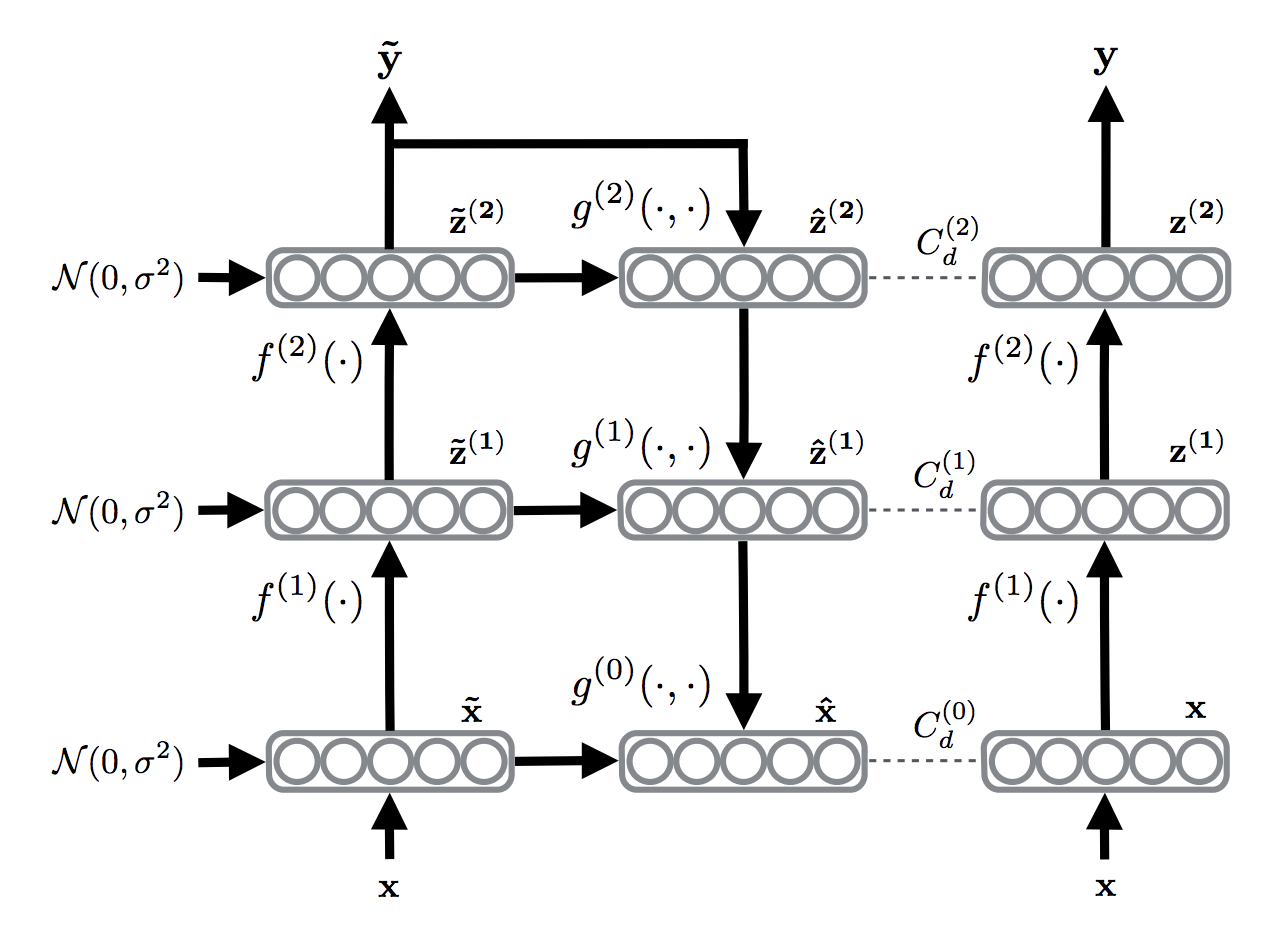
\includegraphics[width=\textwidth]{images/ladder_architecture.png}
\caption{Ilustración conceptual de una red en escalera con L = 2 obtenida del trabajo de \cite{DBLP:journals/corr/RasmusVHBR15}. El camino feedforward $(\textbf{x}\rightarrow\textbf{z}^{(1)}\rightarrow\textbf{z}^{(2)}\rightarrow\textbf{y})$ comparte las asignaciones $f^{(l)}$ con el camino feedforward corrupto, o codificador $(\textbf{x}\rightarrow\tilde{\textbf{z}}^{(1)}\rightarrow\tilde{\textbf{z}}^{(2)}\rightarrow\tilde{\textbf{y}})$. El decodificador $(\tilde{\textbf{z}}^{(l)}\rightarrow\hat{\textbf{z}}^{(l)}\rightarrow\hat{\textbf{x}})$ consiste en las funciones de reducción de ruido $g^{(l)}$ y tiene funciones de costo $C_{d}^{(l)}$ en cada capa, tratando de minimizar la diferencia entre $\hat{\textbf{z}}^{(l)}$ y $\textbf{z}^{(l)}$.
La salida $\tilde{\textbf{y}}$ del codificador también se puede entrenar para que coincida con las etiquetas disponibles $t(n)$. }
\label{fig:ladder_architecture}
\end{center}
\end{figure}


Mientras que las dAE normalmente sólo están capacitadas para reducir el ruido de las observaciones, las DSS se basan en la idea de utilizar funciones de reducción de ruido $\hat{\textbf{z}} = g(\textbf{z})$ de las variables latentes \textbf{z} para entrenar una función $f(\textbf{x}) = \textbf{z}$ que modela la probabilidad de las variables latentes en función de las observaciones. La función de costo es idéntica a la usada en un dAE salvo el hecho de que las variables latentes \textbf{z} reemplazan a las observaciones \textbf{x}; esto es, $\|\hat{\textbf{z}} - \textbf{z}\|^2$. Lo único que hay que tener en cuenta es que \textbf{z} debe normalizarse de alguna manera, ya que de lo contrario el modelo tiene una solución trivial $\textbf{z} = \hat{\textbf{z}} = constante$. En un dAE esto no puede suceder ya que el modelo no puede cambiar la entrada \textbf{x}.

La Figura \ref{fig:ladder_architecture} muestra la estructura de una red en escalera. Cada capa $(l)$ contribuye, a la función de costo $C_{d}$, un término de la forma $C_{d}^{(l)} = \| \textbf{z}^{(l)} - \hat{\textbf{z}}^{(l)}\|^2$ que entrena las capas superiores (tanto codificador como decodificador), para aprender la función de reducción de ruido $\hat{\textbf{z}}^{(l)} = g^{(l)}(\tilde{\textbf{z}}^{(l)},\hat{\textbf{z}}^{(l+1)})$ que asigna el valor corrupto $\tilde{\textbf{z}}^{(l)}$ al estimador de reducción de ruido $\hat{\textbf{z}}^{(l)}$. Como la estimación $\hat{\textbf{z}}^{(l)}$ incorpora todo el conocimiento previo sobre \textbf{z}, el mismo término de función de costo también entrena las capas del codificador, con el objetivo de encontrar características más limpias que coincidan mejor con el valor esperado previo.

Dado que la función de costo necesita tanto lo limpio $\textbf{z}^{(l)}$ como lo corrupto $\tilde{\textbf{z}}^{(l)}$, durante el entrenamiento el codificador se ejecuta dos veces: un pasaje limpio por $\textbf{z}^{(l)}$ y un pasaje corrupto por $\tilde{\textbf{z}}^{(l)}$.

Una forma de visualizar la red en escalera es considerarla como una colección de autoencoders anidados que comparten partes de la maquinaria de reducción de ruido entre sí. Desde el punto de vista del autoencoder en la capa \textit{l}, las representaciones de las capas superiores se pueden tratar como neuronas ocultas. En otras palabras, no hay una razón particular por la cual $\hat{\textbf{z}}^{(l+i)}$ producido por el decodificador, deba parecerse a la correspondiente representación $\textbf{z}^{(l+i)}$ producida por el codificador. Solo la función de costo $C_{d}^{(l+i)}$ los une y obliga a la inferencia a proceder en orden inverso en el decodificador. Este intercambio ayuda a un autoencoder de reducción de ruido profundo a aprender el proceso de reducción de ruido a medida que divide la tarea en subtareas significativas de reducción de ruido en representaciones intermedias.
%     - Ghaddar y Langlais (2017)  -> WiNER: A Wikipedia Annotated Corpus for Named Entity Recognition  -> http://www.aclweb.org/anthology/I17-1042

%     - Zeng M. et al. (2017) -> Semi-Supervised Convolutional Neural Networks for Human Activity Recognition -> https://arxiv.org/pdf/1801.07827.pdf

%     - Iacobacci I. et al. (2016) -> Embeddings for Word Sense Disambiguation: An Evaluation Study -> http://www.aclweb.org/anthology/P16-1085
%     - Rasmus A. et al. (2015) -> Semi-Supervised Learning with Ladder Networks -> https://arxiv.org/abs/1507.02672

\chapter{Entorno de experimentación} \label{chapter:chapter3}

\section{Análisis y procesamiento del corpus}

Siendo el objetivo de este trabajo la evaluación de un método semi-supervisado aplicado al reconocimiento de entidades nombradas se hizo necesario contar con un corpus para realizar dicha tarea. Por ello, se decidió utilizar a WiNER , un corpus anotado a partir de artículos de la Wikipedia en inglés construido en el trabajo de \cite{WiNER-Ghaddar-Langlais}.

Dicho corpus consta de 3.2M de artículos de Wikipedia, que comprende más de 54M de oraciones, de las cuales 41M contienen al menos una anotación de entidad nombrada, generando un total de 106M de anotaciones (un promedio de 2 entidades por oración).

Los tipos de entidades anotadas en este conjunto de datos son PER, LOC y ORG que denotan nombres de personas, lugares y organizaciones respectivamente. También se cuenta con la etiqueta MISC, categoría que incluye aquellas entidades no pertenecientes a las categorías anteriormente mencionadas. \textit{Agatha Christie} (PER), \textit{Belgian} (LOC), \textit{Warner Bros} (ORG) y \textit{Black Coffee} (MISC) son algunos ejemplos de entidades nombradas de este corpus. En caso de que no se trate de una instancia que no corresponde a una entidad nombrada se utiliza, por convención, la etiqueta O.

Una de las primeras decisiones tomadas durante el procesamiento del corpus fue considerar entidades cuya cardinalidad a nivel de palabra fuese uno. Esto se logró separando aquellas entidades formadas por más de una palabra en nuevas entidades donde a cada palabra le corresponde el mismo tipo de entidad de la cual fue separada. En el ejemplo anterior de \textit{Agatha Christie}, ahora se considera \textit{Agatha} y \textit{Christie} como dos entidades independientes, ambas del tipo PER.

El corpus contiene un total de 3223 documentos. El Cuadro \ref{tab:division} muestra la división de datos para conformar los conjuntos de entrenamiento, evaluación y validación.

\begin{table}[ht]
    \centering
    \begin{tabular}{|c|c|}
        \hline
        \textbf{Corpus} & \textbf{Documentos} \\
        \hline \hline
        Entrenamiento & 0 - 1999 \\
        Validación & 2000 - 2599 \\
        Evaluación & 2600 - 3223 \\
        \hline
    \end{tabular}
    \caption{División de los datos para entrenamiento, validación y evaluación.}
    \label{tab:division}
\end{table}

A partir de esa división se tomaron a su vez muestras aleatorias de cada conjunto de documentos detallados en el Capítulo \ref{chapter:chapter4}. Esto fue necesario por cuestiones de limitación de recursos computacionales y tiempo para la ejecución de los distintos experimentos. Se realizó un preprocesamiento sobre los 3223 documentos, cada uno de estos documentos tiene asociado aproximadamente 1000 artículos identificados con un número único. Para cada artículo existe entonces un archivo asociado cuya primera línea tiene su wikiID seguidos de sus oraciones una por línea. En los artículos, los tokens (palabras, símbolos, signos, etc.) están representados por un ID unívoco.

\paragraph{Ejemplo}\hfill

\vspace{0.5em}

\begin{tabular}{|l|}
    \hline
    63903 24730 9 7 3035 4104 7584 1 355 17 22825 9984 2 \\
    \hline
\end{tabular}

\vspace{0.5em}

Es equivalente a:

\begin{tabular}{|l|}
    \hline
    Hercule Poirot is a fictional Belgian detective , created \\
    by Agatha Christie . \\
    \hline
\end{tabular}

\vspace{1em}

Gracias a esta metodología de almacenamiento del corpus no fue necesario aplicar ningún tokenizador sobre el texto. A su vez, se decidió no remover signos de puntuación al igual que las palabras más comunes del idioma \textit{stopwords} con la premisa de que en el caso de removerlas se perdería información útil sobre el contexto de cada palabra para nuestra tarea particular de reconocimiento de entidades nombradas. Una vez realizada la transformación y obtenidas las oraciones, se construyeron las distintas instancias de entrenamiento que se mencionan en la sección \ref{sec:instanciasEntrenamiento}. Finalmente, se encuentran codificadas las entidades de cada artículo. El formato es el siguiente:

\vspace{0.5em}

\begin{tabular}{|l|}
    \hline
    ID $<$wikiID$>$ \\
    sentIdx begin end entityType \\
    \hline
\end{tabular}

\vspace{1em}

Donde \textit{sentIdx} representa el número de oración del artículo, \textit{begin} la posición donde comienza una entidad en la oración, \textit{end} la posición donde termina y \textit{entityType} el tipo de entidad que se trata:

\vspace{0.5em}

\begin{tabular}{|ll|}
    \hline
    entityType[0] = PER & entityType[1] = LOC \\
    entityType[2] = ORG & entityType[3] = MISC \\
    \hline
\end{tabular}

\vspace{1em}

Continuando el ejemplo anterior:

\vspace{0.5em}

\begin{tabular}{|llll|}
    \hline
    ID & 1000 & & \\
    0 & 0 & 2 & 0 \\
    0 &	5 &	6 & 1 \\
    0 &	10 & 12 & 0 \\
    \hline
\end{tabular}

\vspace{1.0mm}

Resulta en:

\vspace{0.5em}

\begin{tabular}{|l|}
    \hline
    [Hercule Poirot]$_{PER}$ is a fictional [Belgian]$_{LOC}$ detective , \\
    created by [Agatha Christie]$_{PER}$ . \\
    \hline
\end{tabular}

\section{Instancias de entrenamiento}
\label{sec:instanciasEntrenamiento}

En este trabajo se exploraron tres maneras de representar a los datos en los
modelos de aprendizaje.

\subsection{Palabra - etiqueta}\label{sec:palabraEtiqueta}

En este caso se hizo necesario investigar metodologías que nos permitieran representar a una palabra teniendo el cuenta el contexto en el cual ocurre. Como primera medida, se decidió utilizar los \textit{embeddings} pre-entrenados de Google\footnote{\url{https://code.google.com/archive/p/word2vec/}} para transformar a cada palabra en un vector que la representa en un espacio de dimensionalidad igual a 300.

Siguiendo el trabajo de \cite{iacobacci-etal-2016-embeddings} se exploraron cuatro estrategias distintas para obtener una representación más informativa de cada palabra.

\subsubsection{Concatenación}
Este método consiste en concatenar los vectores de palabras que rodean una palabra objetivo en un vector más grande, que tiene un tamaño igual a las dimensiones sumadas de todas las proyecciones (\textit{embeddings}) individuales.

\begin{itemize}
    \item $w_{ij}$ = peso asociado con la i-ésima dimensión del vector de la j-ésima palabra en la oración. Con los vectores de palabras de una oración se forma una matriz $w^{\space D\space x\space L}$ donde $L$ es la cantidad de palabras de esa oración.
    \item $D$ = dimensionalidad de los word vectors originales. Por ejemplo, al usar el modelo Word2Vec de Google se tiene $D$ = 300.
    \item $W$ = tamaño de ventana que se define como el número de palabras en un solo lado.
\end{itemize}

Nos interesa representar el contexto de la I-ésima palabra de la oración. La i-ésima dimensión del vector de concatenación, que tiene un tamaño de $2 W D$, se calcula de la siguiente manera:

$$e_{i} =\begin{cases} 
      w_{i \; mod \; D,\;\; I \; - \; W \; + \; \left\lfloor{\frac{i}{D}}\right\rfloor} & \left\lfloor{\frac{i}{D}}\right\rfloor < W \\
      w_{i\; mod \; D,\;\; I \; - \; W \; + \; 1\;  +\;\left\lfloor{\frac{i}{D}}\right\rfloor} & c.c.
   \end{cases}$$

Al tomar una ventana simétrica, se realiza un relleno (\textit{padding}) con ceros a izquierda y/o derecha según corresponda para mantener la misma dimensionalidad en cada nuevo vector generado.

\subsubsection{Promedio}

Como su nombre indica, se calcula el centroide de los embeddings de todas las palabras circundantes. La fórmula divide cada dimensión en $2W$ ya que el número de palabras del contexto es dos veces el tamaño de la ventana:

$$e_{i} =\sum_{\substack{j\;=\; I-W \\ j\;\neq\; I}}^{I + W} \frac{w_{ij}}{2W}$$

\subsubsection{Decaimiento fraccional}
Una tercera estrategia para construir un vector de características en base a los embeddings de palabras contextuales está inspirada en la forma en que Word2vec combina las palabras en el contexto. Aquí, se supone que la importancia de una palabra para nuestra representación es inversamente proporcional a su distancia respecto a la palabra objetivo.

Por lo tanto, las palabras contextuales se ponderan en función de su distancia de la palabra objetivo:

$$e_{i} =\sum_{\substack{j\;=\; I-W \\ j\;\neq\; I}}^{I + W} w_{ij} *\frac{W - \lvert I-j\rvert}{W}$$

\subsubsection{Decaimiento exponencial}
Funciona de manera similar al decaimiento fraccional, que le da más importancia al contexto cercano, pero en este caso la ponderación se realiza exponencialmente:

$$e_{i} =\sum_{\substack{j\;=\; I-W \\ j\;\neq\; I}}^{I + W} w_{ij} * (1 - \alpha)^{\lvert \; I\;-\; j\;\rvert\;-\;1}$$

donde $\alpha = 1 - 0.1^{(W-1)^{-1}}$ es el parámetro de decaimiento. Se elige el parámetro de tal manera que las palabras inmediatas que rodean a la palabra objetivo contribuyen 10 veces más que las últimas palabras en ambos lados de la ventana.

\subsection{Fragmento de oración - etiqueta}\label{sec:fragmento_sentencia}

Para la aplicación de capas convolucionales la entrada del modelo deja de ser solo una palabra. Una primera alternativa fue tomar fragmentos de oraciones donde la palabra ubicada en el centro es la palabra a clasificar. Se decidió tomar una ventana simétrica de 2 palabras a izquierda y derecha de la palabra objetivo con la premisa de que el contexto relevante para la tarea de clasificación de la palabra objetivo son aquellas palabras de ocurrencia cercana. Para mayor claridad, un ejemplo de esto puede observarse en el Cuadro \ref{tab:fragmento:oracion}.

\begin{table}[ht]
    \centering
    \begin{tabular}{|l|c|}
        \hline
        \textbf{Contexto} & \textbf{Etiqueta} \\
        \hline
        ['It', 'aired', '\textbf{on}', 'NBC', 'from'] & O \\\relax
        ['aired', 'on', '\textbf{NBC}', 'from', 'February'] & ORG \\\relax
        ['on', 'NBC', '\textbf{from}', 'February', '2002'] & O \\\relax
        ['NBC', 'from', '\textbf{February}', '2002', 'to'] & MISC \\\relax
        ['from', 'February', '\textbf{2002}', 'to', 'May'] & MISC \\\relax
        ['February', '2002', '\textbf{to}', 'May', '2003'] & O \\
        \hline
    \end{tabular}
    \caption{Ejemplo de fragmentos de oración y etiquetas respectivas al contexto.}
    \label{tab:fragmento:oracion}
\end{table}

La información sobre el contexto de la palabra objetivo será obtenida entonces a partir de la aplicación de capas convolucionales sobre el fragmento en cuestión.

\subsection{Oración - etiquetas}\label{sec:sequence_labeling}

En aprendizaje automático, el etiquetado de secuencias, del inglés \textit{sequence labeling}, es un tipo de tarea que implica la asignación de una etiqueta categórica a cada miembro de una secuencia de valores observados.

El etiquetado de secuencias es una aproximación clásica cuando se trata de lidiar con reconocimiento de entidades en particular (y otras tareas de PLN en general). Esto es así porque la disposición de las palabras en el lenguaje natural es inherentemente secuencial, muchas veces una palabra hace referencia a un hecho que sucedió anteriormente en el texto y se quiere que el modelo de aprendizaje automático capture esa información siendo idóneo que la entrada del mismo sea una secuencia.

Debido a que la entrada del modelo debe que ser un vector de longitud fija se hizo necesario determinar un tamaño máximo para las oraciones. Se observó entonces la distribución de la cantidad de palabras por oración y se decidió tomar sentencias de longitud igual a 30. Como consecuencia, se truncan aquellas oraciones de longitud mayor a 30 y se completan con 0's a derecha aquellas cuya longitud es menor.

\begin{table}[ht]
    \centering
    \begin{tabular}{|l|c|}
        \hline
        \textbf{Secuencia} \\
        \hline
        ['It', 'aired', 'on', 'NBC', 'from', 'February', '2002', 'to', 'May', '2003', '.'] \\
        \hline
        \textbf{Etiquetas} \\
        \hline
        [O, O, O, ORG, O, MISC, MISC, O, MISC, MISC, O] \\
        \hline
    \end{tabular}
    \caption{Ejemplo de oración y etiquetas.}
    \label{tab:fragmento:oracion}
\end{table}

\section{Métricas de evaluación}

Una de las métricas más conocidas para la evaluación de modelos de aprendizaje automático en problemas de clasificación es la exactitud (del inglés \textit{accuracy}). Esta métrica en particular cuenta la cantidad de aciertos que tuvo el modelo a la hora de clasificar un dato de entrada y la divide sobre el total de datos clasificados. Se entiende por acierto cada vez que el modelo predice la etiqueta correcta para un dato ingresado. Más formalmente, en un problema de clasificación binaria con dos clases Positivo y Negativo:

% \[
% \text{Exactitud} = \frac{Verdadero Positivos + Verdadero Negativos}{Verdadero Positivos + Verdadero Negativos + Falso Positivos + Falso Negativos}
% \]
\[
\text{Exactitud (accuracy)} = \frac{TP + TN}{TP + TN + FP + FN}
\]

Donde: 

\vspace{5.0mm}

$TP$ = \textit{True Positive} o Verdaderos Positivos

\vspace{1.0mm}

$TN$ = \textit{True Negatives} o Verdaderos Negativos

\vspace{1.0mm}

$FP$ = \textit{False Positives} o Falsos Positivos

\vspace{1.0mm}

$FN$ = \textit{False Negatives} o Falsos Negativos

\vspace{5.0mm}

Esta definición se extiende fácilmente a un problema de más de dos clases.

La exactitud es una métrica estándar, pero tiene algunos defectos a la hora de ser utilizada para evaluar un modelo. En particular, está muy sesgada para los casos de clases desbalanceadas.

Muchas veces puede ocurrir que la distribución de las clases en un conjunto de datos observado no es homogénea, sino por el contrario se encuentra muy desbalanceada. Esto es especialmente común en tareas de lenguaje natural por lo que se conoce como \textit{Ley de Zipf} \cite{j:zpf}.

Tomando como ejemplo un problema de clasificación binaria, supongamos que nuestra muestra contiene 100 ejemplos de entrenamiento de los cuales 99 pertenecen a la clase negativa y sólo 1 a la clase positiva. Un modelo muy sencillo que sin importar el dato de entrada siempre lo clasifique como negativo obtendrá un valor de \textit{accuracy} de 0.99 pero este modelo nunca va a ser capaz de clasificar correctamente un dato perteneciente a la clase positiva. Si bien existen maneras para tratar el desbalance de clases, existen a su vez otras métricas que nos dan más confiabilidad respecto al desempeño del modelo en este escenario.

Por un lado tenemos la métrica \textit{recall} que mide la capacidad de un modelo para encontrar todos los casos relevantes dentro de un conjunto de datos. Entendamos casos relevantes como aquellos pertenecientes a una clase en particular, i.e. la clase positiva. Formalmente se define como:

\[
\text{Recall} = \frac{TP}{TP + FN}
\]

\vspace{5.0mm}

Por otro lado tenemos la métrica \textit{precision} que expresa la proporción de los datos que nuestro modelo dice que eran relevantes (positivos) realmente eran relevantes. Para esto, se tienen en cuenta los falsos positivos, es decir, la cantidad de veces que el modelo de manera incorrecta etiquetó como positivo un dato que era en realidad negativo. Formalmente se define como: 

\[
\text{Precision} = \frac{TP}{TP + FP}
\]

\vspace{5.0mm}

Finalmente, existe una métrica que representa la media armónica entre las anteriores:

\[
\text{F1-score} = \frac{2 \cdot precision\cdot recall}{precision + recall}
\]

\vspace{5.0mm}

Notar que esta métrica penaliza valores extremos. Por ejemplo, con una \textit{precision} igual a 0 y una \textit{recall} igual a 1 el \textit{f1-score} resulta igual a 0 mientras que con solo tomar el promedio se obtiene un valor igual a 0.5 que no representa bien la combinación de las métricas anteriores.

Una característica fundamental que un buen modelo de aprendizaje automático debe poseer es la \textit{generalización}. Entendemos por generalización la capacidad que tiene el modelo de obtener buenos resultados con datos nuevos, es decir, el modelo también debe ajustarse de manera correcta a aquellos datos que no se utilizaron para el entrenamiento del mismo. Para medir entonces que tan bien generaliza un modelo es una convención realizar una división de los datos en tres conjuntos: entrenamiento, validación y test. A partir de esto, se analiza que tanto difieren los resultados de performance del modelo para cada conjunto de datos. Mientras menor sea la diferencia entre los datos en entrenamiento y los datos nuevos (validación y test) podemos afirmar que el modelo posee mayor capacidad de generalizar.

Otra manera más robusta de medir la generación es utilizar lo que se conoce como \textit{validación cruzada} (del inglés, \textit{cross-validation}). Cuando usamos los conjuntos de entrenamiento y validación, hay una parte aleatoria que puede influir los resultados. Dependiendo cómo dividamos los datos en estos dos conjuntos tendremos una estimación diferente del error de generalización. En unos casos pensaremos que el modelo generaliza mejor y en otros peor. Para combatir este problema, la validación cruzada propone crear los conjuntos de entrenamiento y validación varias veces, cada vez con una separación diferente. De esta forma obtendremos estimaciones diferentes. La media de todos los errores de validación se considera la estimación del error de generalización. Es una estimación más robusta. El inconveniente es que es computacionalmente más costoso. La solución de compromiso es usar validación cruzada pero limitar el número de veces que la hacemos.


\section{Arquitectura de los modelos}

\subsection{Perceptron Multicapa}\label{sec:perceptron}

El modelo Perceptrón Multicapa (MLP) es una red neuronal artificial del tipo \textit{feed-forward} \cite{Hornik:1989:MFN:70405.70408}. Consiste en un grafo dirigido de múltiples capas, cada capa contiene una cantidad variable de nodos los cuales están totalmente conectados con los nodos de capa anterior y/o posterior según corresponda. En la Figura \ref{fig:MLP_architecture} se observa un ejemplo de este tipo de red donde cada nodo adquiere el nombre de neurona que aplica una función de activación no lineal. De esta manera, su composición le brinda la capacidad de distinguir datos de naturaleza no linealmente separables, limitación que sufren modelos de aprendizaje más tradicionales.

%Figura MLP architecture
\begin{figure}[ht]
\begin{center}
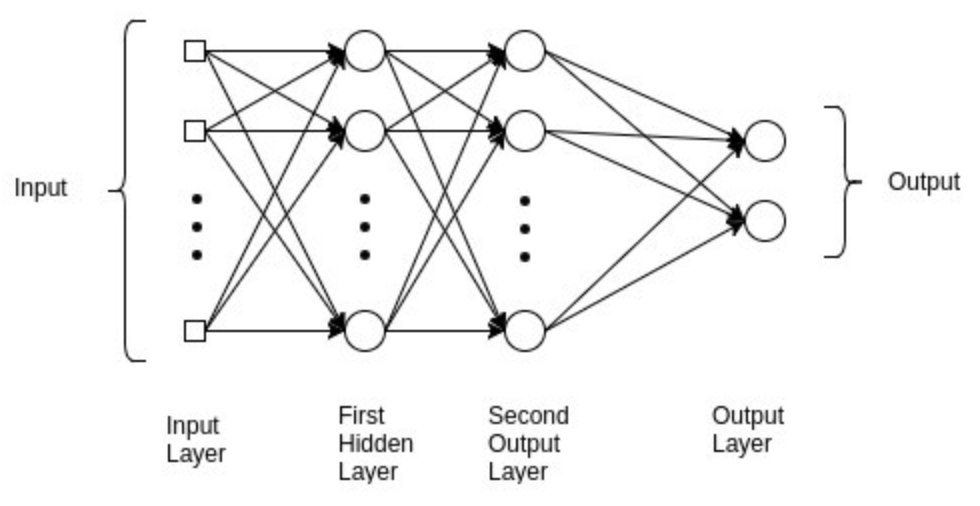
\includegraphics[width=.9\linewidth]{images/MLP_architecture.png}
\caption{Ejemplo de una red neuronal perceptron multicapa.}
\label{fig:MLP_architecture}
\end{center}
\end{figure}

Se decidió utilizar este modelo a modo de \textit{baseline}, y para determinar cuál estrategia de representación de palabras del trabajo de \cite{iacobacci-etal-2016-embeddings} funcionaba mejor. La capa de entrada del modelo toma una palabra representada a través de un vector, resultante de haber aplicado alguna de las estrategias citadas en la sección \ref{sec:palabraEtiqueta}. La capa de salida contiene cinco neuronas, ya que se cuenta con cinco clases: PER - LOC - ORG - MISC - O, posteriormente se aplica la función de activación softmax que asigna la salida no normalizada a una distribución de probabilidad sobre las clases de salida.

\subsection{Redes convolucionales en amplitud}\label{sec:cnn:wide}

\begin{figure}[ht!]
\begin{center}
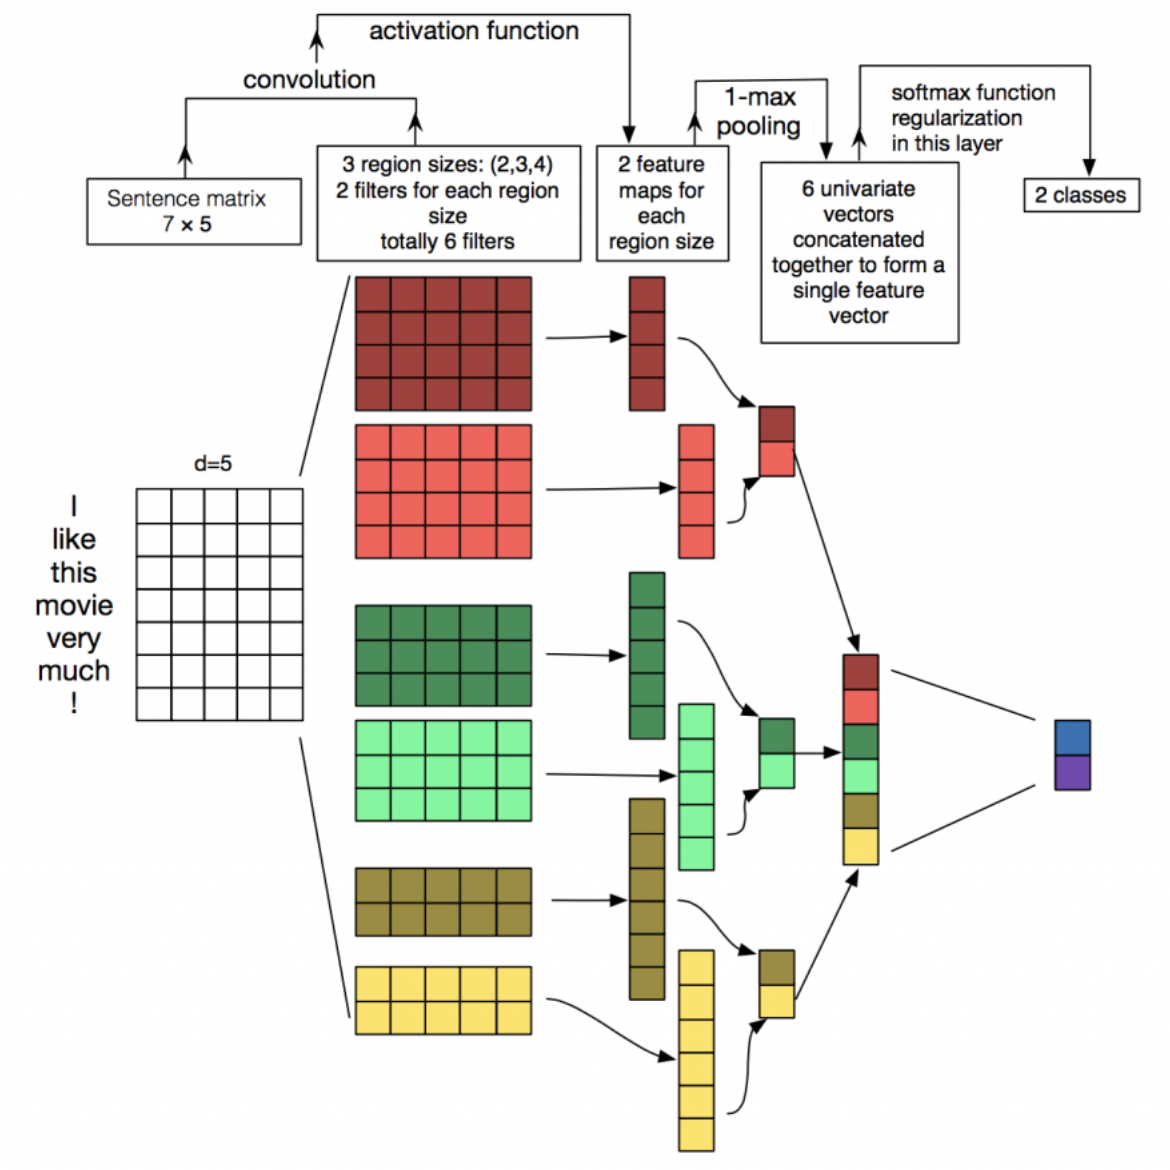
\includegraphics[width=.9\linewidth]{images/CNN_wide_NLP.png}
\caption{Ejemplo de una red convolucional en amplitud para análisis de sentimiento.}
\label{fig:CNN_wide_architecture}
\end{center}
\end{figure}

La entrada de la mayoría de los modelos que realizan tareas de procesamiento de lenguaje natural son oraciones o documentos representados en una matriz. Cada fila de la matriz corresponde a un \textit{token}, típicamente una palabra, pero también podría ser un carácter, representado a través de un vector.

Al aplicar los filtros de las convoluciones, usualmente los mismos se deslizan sobre las filas completas de la matriz (palabras). Por lo tanto, el ancho de nuestros filtros suele ser el mismo que el ancho de la matriz de entrada. La altura es lo que puede variar, tomando ventanas de \textit{n} palabras a la vez.

La Figura \ref{fig:CNN_wide_architecture} muestra un ejemplo de esta arquitectura\footnote{\url{http://www.wildml.com/2015/11/understanding-convolutional-neural-networks-for-nlp/}}. Se toman filtros de alturas 2, 3 y 4 y se supone un \textit{stride} (desplazamiento del filtro en cada paso) igual a 1. Luego de la convolución se aplica una función de activación y se obtienen distintos vectores que contienen información sobre la sentencia original. Posteriormente se aplica una capa de \textit{max pooling} cuyo objetivo es reducir la dimensionalidad pero con la promesa de mantener la información más relevante. Finalmente se construye un único vector al concatenar los vectores resultantes y se aplica una función de activación softmax a la capa densa de salida para realizar la clasificación correspondiente.

\subsection{Redes convolucionales en profundidad}\label{sec:cnn:deep}

Una alternativa al modelo de redes convolucionales en amplitud que también le permite a las representaciones intermedias obtener información sobre el contexto de la sentencia es el modelo de redes convolucionales en profundidad.

La idea es hacer crecer el campo receptivo a medida que se apilan más y más capas convolucionales. Esto significa que, de forma predeterminada, cada paso en la representación de la convolución ve toda la entrada en su campo receptivo.

En la Figura \ref{fig:CNN_depth_architecture} se puede ver como al agregar más capas se incrementa el campo receptivo\footnote{\url{https://medium.com/@TalPerry/convolutional-methods-for-text-d5260fd5675f}}. Esto significa que dada una profundidad suficiente, nuestra red podría mirar toda la capa de entrada, a través de unas pocas abstracciones.

\begin{figure}[hb]
\begin{center}
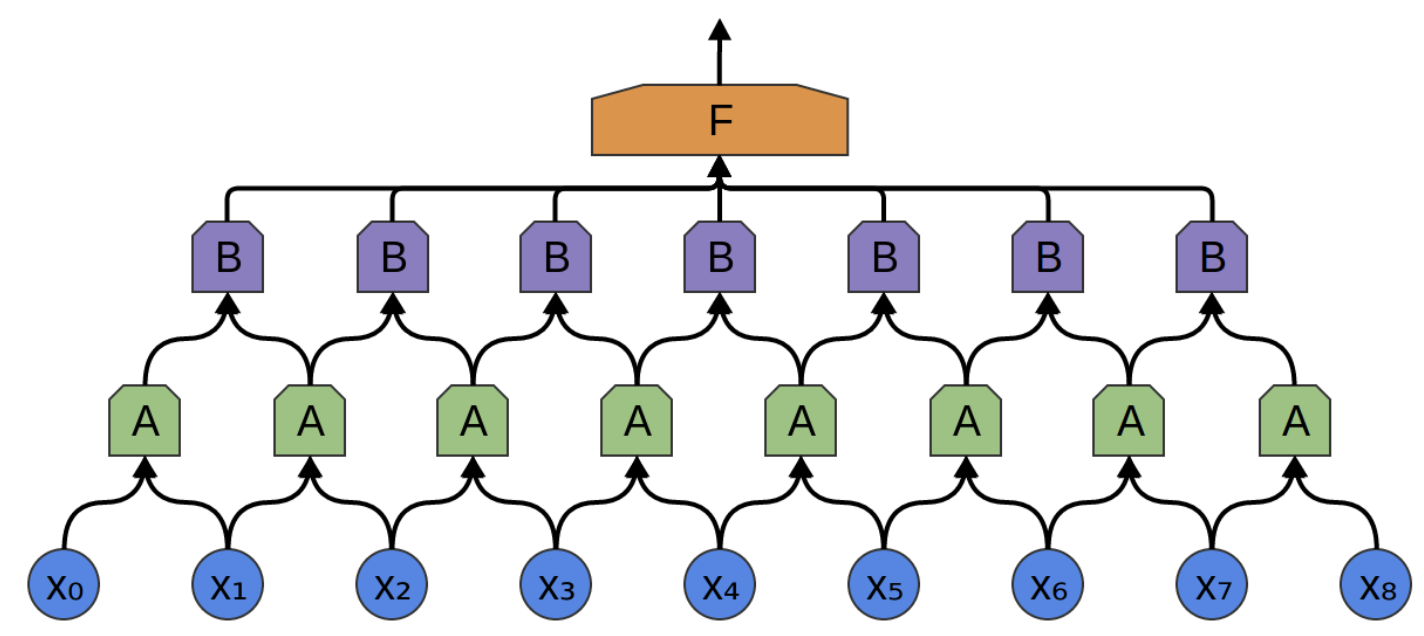
\includegraphics[width=.9\linewidth]{images/CNN_depth_NLP.png}
\caption{Ejemplo de una red convolucional en profundidad.}
\label{fig:CNN_depth_architecture}
\end{center}
\end{figure}

\subsection{Redes neuronales en escalera}\label{sec:ladder_net}

La idea detrás de las redes neuronales en escalera es entrenar simultáneamente una red neuronal del tipo 
\textit{feed-forward} (como lo son la red perceptrón multicapa y las redes convolucionales) junto con un 
autoencoder con pesos compartidos. La red se entrena aprendiendo dos objetivos diferentes: uno supervisado, 
dado por el error de predicción de los datos etiquetados; y otro no supervisado, dado por el error de 
reconstrucción de los datos sin etiquetar.

En el presente trabajo, se exploró el uso de un parámetro extra sobre la función de costo de la red en escalera original. Al factor no supervisado de la función de costo se lo multiplica por un parámetro $\mu$ que viene a representar la relevancia de la tarea no supervisada en el modelo. La función de costo final es:

\[
Cost = \text{supervised\_cost} + \mu ~ \text{unsupervised\_cost}
\]

La estructura del modelo es un autoencoder con \textit{skip connections} desde el codificador hacia 
el decodificador y la tarea de aprendizaje es similar a los autoencoders de eliminación de ruido popularmente 
conocidos como \texit{denoising autoencoders} pero en este caso dicha tarea se aplica a cada capa, no solo a 
las entradas. Las \textit{skip connections} liberan la presión de representar  los detalles en las capas más 
altas del modelo porque a través de estas conexiones el decodificador puede recuperar cualquier detalle 
descartado por el codificador. Una descripción más detallada de este modelo se encuentra en la sección 
\ref{sec:related_work_ladder} como así también remitimos al lector a \cite{DBLP:journals/corr/RasmusVHBR15}.

% \section{Análisis y pre-procesamiento del corpus}
% \section{Implementación de la red convolucional en escalera}

\chapter{Experimentación y análisis de resultados} \label{chapter:chapter4}

\section{Baselines supervisados}

Previo a la experimentación con los modelos de redes convolucionales en escalera, era necesario buscar
un punto de comparación de estos modelos con algún baseline. Por lo cuál, se seleccionaron tres baselines
basándonos en una estructura de red neuronal puramente supervisada, es decir, sin utilizar datos no anotados como es el caso de la red en escalera. Estos se detallaron en el Capítulo anterior, y 
a continuación se denotarán los experimentos y mostrarán los resultados de los mismos.

\subsection{Perceptrón multicapa}\label{baseline:mlp}

El primer conjunto de experimentos fue realizado sobre el perceptrón multicapa común, que se describe con 
mayor detalle en la Sección \ref{sec:perceptron}. El conjunto de datos para entrenamiento y evaluación de este
modelo se establecieron en 100000 instancias de entrenamiento y 20000 para evaluación y validación. Para 
conseguir esta muestra de ejemplos primero se realizó una división de los documentos del corpus como se 
detalla en el Cuadro \ref{tab:division}. 

Luego, sobre cada subconjunto de documentos se tomo una muestra aleatoria de las instancias mencionadas 
anteriormente. 

Notar que para estas muestras se realizó un \textit{subsampling} de la clase O tanto para las instancias de
tipo \textit{palabra-etiqueta} como para \textit{fragmento oración-etiqueta}. Esta decisión fue tomada con el
objetivo de balancear las clases.

Para el caso del perceptrón multicapa se muestran tres experimentos, uno para cada estrategia de 
representación, con los hiperparámetros que mejores resultados obtuvieron seleccionados de manera aleatoria.
Estos pueden verse detallados en el Cuadro \ref{tab:exp:perceptron}.

\begin{table}[h]
    \centering
    \begin{tabular}{|l|l|l|}
        \hline
        \textbf{Experimento} & \textbf{Hiperparámetro} & \textbf{Valor} \\
        \hline
        \multirow{4}{*}{MLP.1} & Representación & Promedio \\
                               & Ventana & 5 \\
                               & Capas & [300, 256, 128, 5] \\
                               & Tasa de aprendizaje & 0.3 \\
        \hline
        \multirow{4}{*}{MLP.2} & Representación & Decaimiento fraccional \\
                               & Ventana & 5 \\
                               & Capas & [300, 256, 128, 5] \\
                               & Tasa de aprendizaje & 0.3 \\
        \hline
        \multirow{4}{*}{MLP.3} & Representación & Decaimiento exponencial \\
                               & Ventana & 5 \\
                               & Capas & [300, 256, 128, 5] \\
                               & Tasa de aprendizaje & 0.3 \\
        \hline
    \end{tabular}
    \caption{Hiperparámetros del conjunto de experimentos con perceptrón multicapa supervisado.}
    \label{tab:exp:perceptron}
\end{table}

\subsubsection{Resultados}

La Figura \ref{fig:MLPbaselines} muestra los resultados de aplicar los tres experimentos detallados en el
Cuadro \ref{tab:exp:perceptron}. Es un gráfico de barras con agrupación. El eje $y$ del gráfico muestra la
exactitud ({\em accuracy}) del experimento, donde a mayor valor, mejor el resultado. 

Por otro lado, el eje $x$ representa la estrategia aplicada (i.e. el experimento de acuerdo al Cuadro 
\ref{tab:exp:perceptron}), agrupando tres barras de acuerdo al conjunto de datos sobre el que se muestra el 
resultado. De esta manera, la barra azul muestra el resultado sobre el conjunto de entrenamiento, la barra 
naranja sobre el conjunto de validación y la barra verde sobre el conjunto de evaluación ({\em test}).

\begin{figure}[t]
\begin{center}
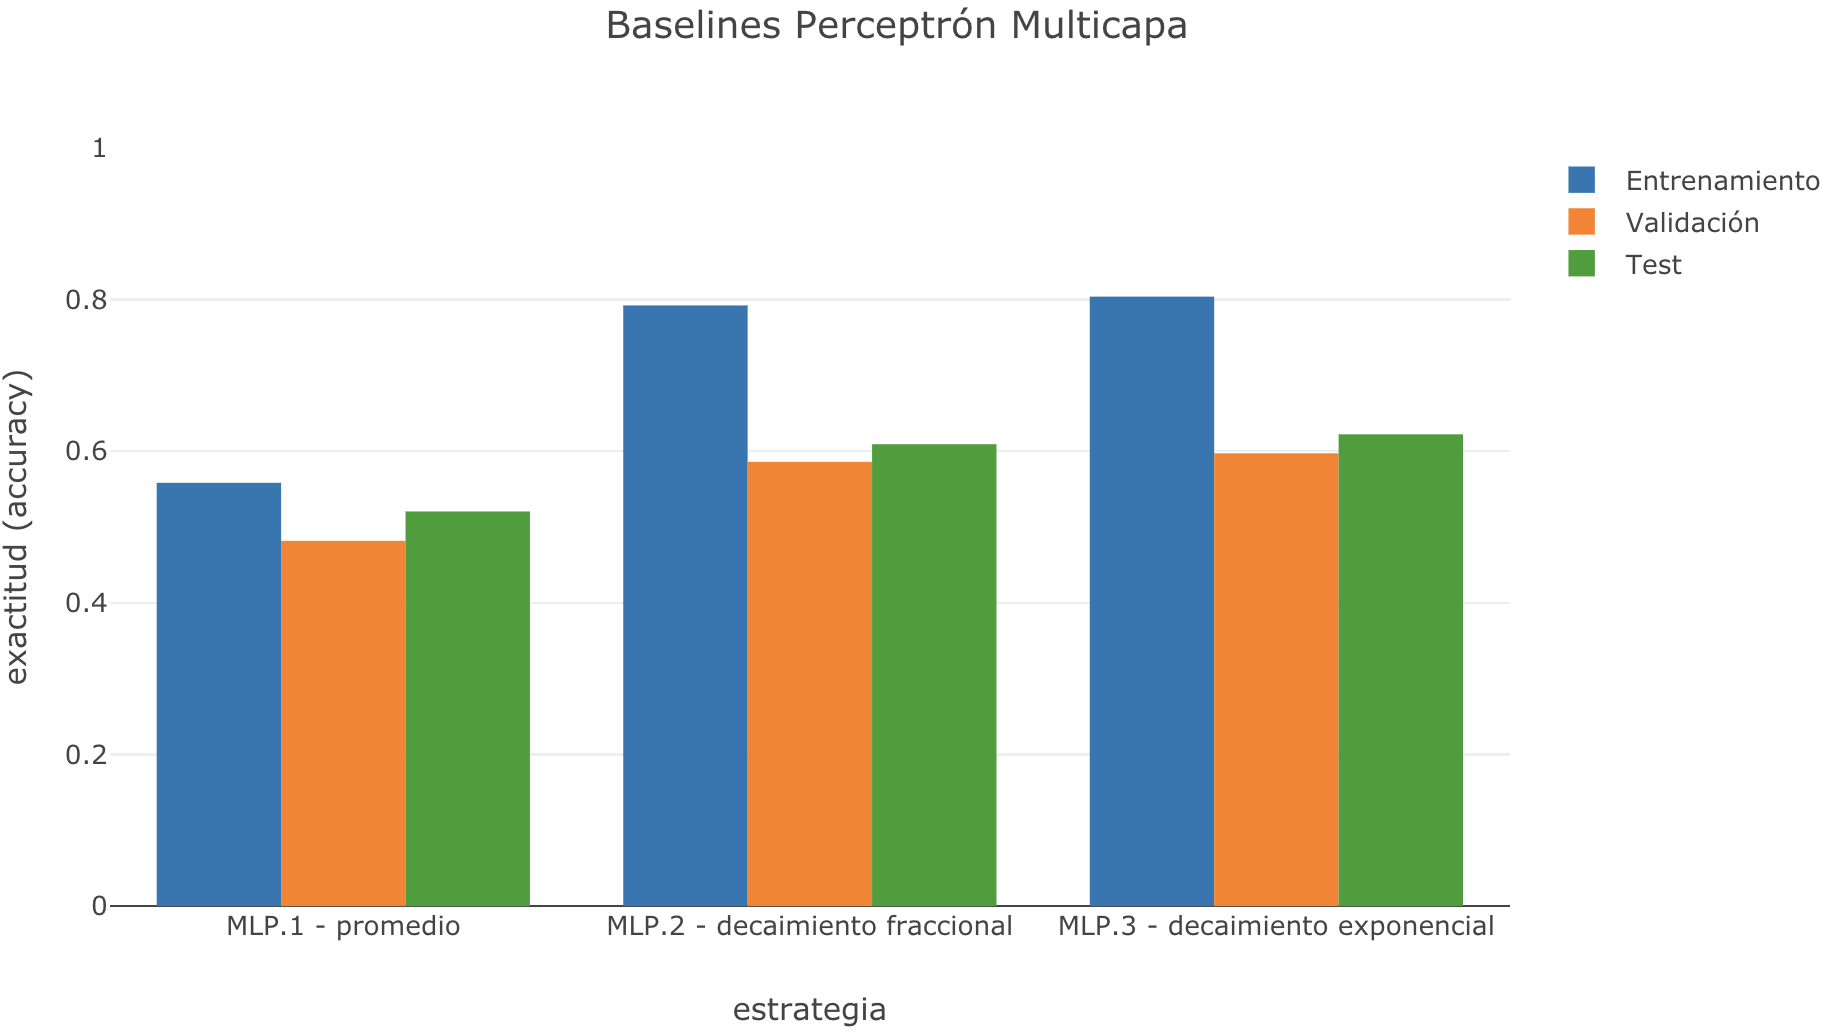
\includegraphics[width=.9\linewidth]{images/MLP_baselines.png}
\caption{Resultados de los experimentos MLP. Comparación utilizando distintas representaciones de datos de 
entrada.}
\label{fig:MLPbaselines}
\end{center}
\end{figure}

Como se puede observar en la Figura \ref{fig:MLPbaselines}, utilizar el decaimiento exponencial y fraccional 
como estrategias de representación de una palabra son una buena alternativa. 

Esto posiblemente se deba a que la información de contexto que le aporta una palabra inmediatamente vecina a 
la palabra objetivo es mucho más relevante que una más distante. 

Por otro lado, simplemente tomar el promedio de las palabras circundantes no tiene buenos resultados y 
justamente no tiene en cuenta lo mencionado anteriormente. De estos experimentos el experimento MLP.3 es el 
que mejor resultados obtiene y es el seleccionado para su comparación en los experimentos mostrados en las 
siguientes secciones.

\subsection{Redes convolucionales en amplitud}\label{baseline:cnn:wide}

Para estos experimentos un ejemplo de entrenamiento es un fragmento de oración como se detalla en la Sección 
\ref{sec:fragmento_sentencia}. 

El conjunto de datos para el entrenamiento y evaluación de este modelo se establecieron 100000 instancias de 
entrenamiento y 20000 para validación y evaluación de manera análoga a los experimentos anteriores. 

El Cuadro \ref{tab:exp:cnn_wide_supervised} establece la lista de experimentos e hiperparámetros utilizados. 
El objetivo los experimentos es analizar si el modelo sufre variaciones al utilizar diferentes proporciones de
instancias de entrenamiento anotadas.

\begin{table}[h]
    \centering
    \begin{tabular}{|l|l|l|}
        \hline
        \textbf{Experimento} & \textbf{Hiperparámetro} & \textbf{Valor} \\
        \hline
        \multirow{7}{*}{Hiper. generales} & Ventana simétrica W & 2 \\
                              & Número de filtros & 100 \\
                              & Tamaño de max pooling & 1 \\
                              & Tamaño de kernels & [2,3,4] \\
                              & Dropout & 0.5 \\
                              & Capas densas & [128, 5] \\
                              & Regularizador L2 & 1 \\
        \hline
        \multirow{1}{*}{CNN-Wide-Sup.1} & \% ejemplos entrenamiento & 25\% \\
        \hline
        \multirow{1}{*}{CNN-Wide-Sup.2} & \% ejemplos entrenamiento & 50\% \\
        \hline
        \multirow{1}{*}{CNN-Wide-Sup.3} & \% ejemplos entrenamiento & 75\% \\
        \hline
        \multirow{1}{*}{CNN-Wide-Sup.4} & \% ejemplos entrenamiento & 100\% \\
        \hline
    \end{tabular}
    \caption{Hiperparámetros para CNN Supervisado en Amplitud.}
    \label{tab:exp:cnn_wide_supervised}
\end{table}

\subsubsection{Resultados}

La Figura \ref{fig:CNN_wide_baselines_ratios} muestra los resultados de aplicar los cuatro experimentos 
detallados en el Cuadro \ref{tab:exp:cnn_wide_supervised}. Se observan las curvas correspondientes al valor de
exactitud que logra cada modelo a lo largo de las épocas de entrenamiento. Se utiliza el color azul para 
denotar la exactitud en los datos de entrenamiento mientras que el anaranjado para los datos de validación. No
se observan diferencias significativas al utilizar una menor cantidad de datos anotados para el entrenamiento 
del modelo. Más adelante se tendrá en consideración el experimento CNN-Wide-Sup.4 que utiliza el 100\% de las 
instancias de entrenamiento para su comparación con el equivalente en la versión en escalera.

\begin{figure}[t]
\begin{center}
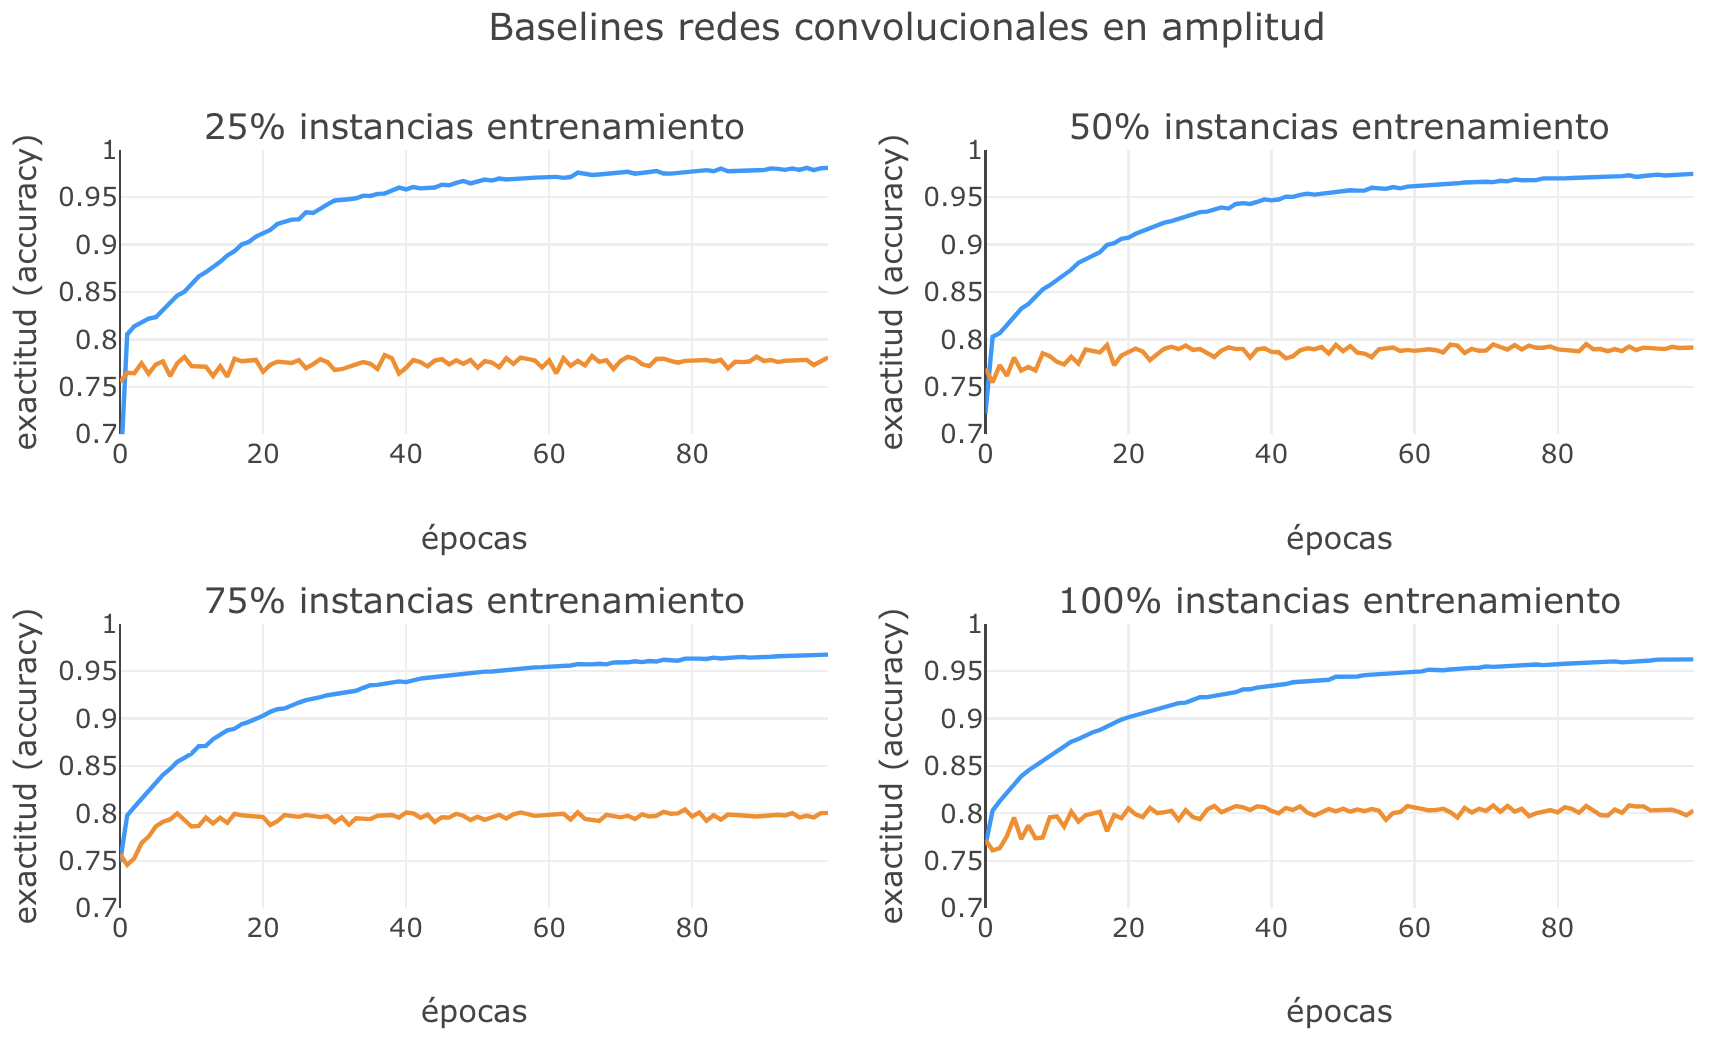
\includegraphics[width=.9\linewidth]{images/CNN_wide_baselines_ratios.png}
\caption{Resultados redes convolucionales en amplitud. Comparación utilizando distintas porciones de corpus
como datos de entrenamiento para el modelo.}
\label{fig:CNN_wide_baselines_ratios}
\end{center}
\end{figure}

\subsection{Redes convolucionales en profundidad}\label{baseline:cnn:deep}

Para estos experimentos la entrada del modelo es una oración y la salida una secuencia de etiquetas que se 
corresponde una a una con cada \textit{token} de la oración ingresada tal como se detalla en la Sección 
\ref{sec:sequence_labeling}. 

El conjunto de datos para el entrenamiento y evaluación de este modelo se establecieron 100000 instancias de 
entrenamiento y 20000 para validación y evaluación. Para este caso en el que las instancias son oraciones y no
palabras no se realiza un \textit{subsampling} de la clase mayoritaria O, por lo que el conjunto de datos se 
presenta inherentemente desbalanceado. 

Para el caso del modelo de redes convolucionales en profundidad supervisado se muestran cuatro experimentos, 
con los hiperparámetros que mejores resultados obtuvieron seleccionados de manera aleatoria. En particular, se
busca ver si el uso de varias capas convolucionales mejora el desempeño del modelo. Estos pueden verse 
detallados en el Cuadro \ref{tab:exp:cnn_depth_supervised}.

\begin{table}[h]
    \centering
    \begin{tabular}{|l|l|l|}
        \hline
        \textbf{Experimento} & \textbf{Hiperparámetro} & \textbf{Valor} \\
        \hline
        \multirow{3}{*}{Hiper. generales} & Tamaño de kernels & 2 \\
                              & Dropout & 0 \\
                              & Regularizador L2 & 0 \\
        \hline
        \multirow{2}{*}{CNN-Depth-Sup.1} & Capas convolucionales & 3 \\
                                         & Número de filtros por capa & 50 \\
        \hline
        \multirow{2}{*}{CNN-Depth-Sup.2} & Capas convolucionales & 10 \\
                                         & Número de filtros por capa & 50 \\
        \hline
        \multirow{2}{*}{CNN-Depth-Sup.3} & Capas convolucionales & 3 \\
                                         & Número de filtros por capa & 100 \\
        \hline
        \multirow{2}{*}{CNN-Depth-Sup.4} & Capas convolucionales & 5 \\
                                         & Número de filtros por capa & 100 \\
        \hline
    \end{tabular}
    \caption{Hiperparámetros del conjunto de experimentos con redes convolucionales en profundidad 
    supervisado.}
    \label{tab:exp:cnn_depth_supervised}
\end{table}

\subsubsection{Resultados}

\begin{figure}[t]
\begin{center}
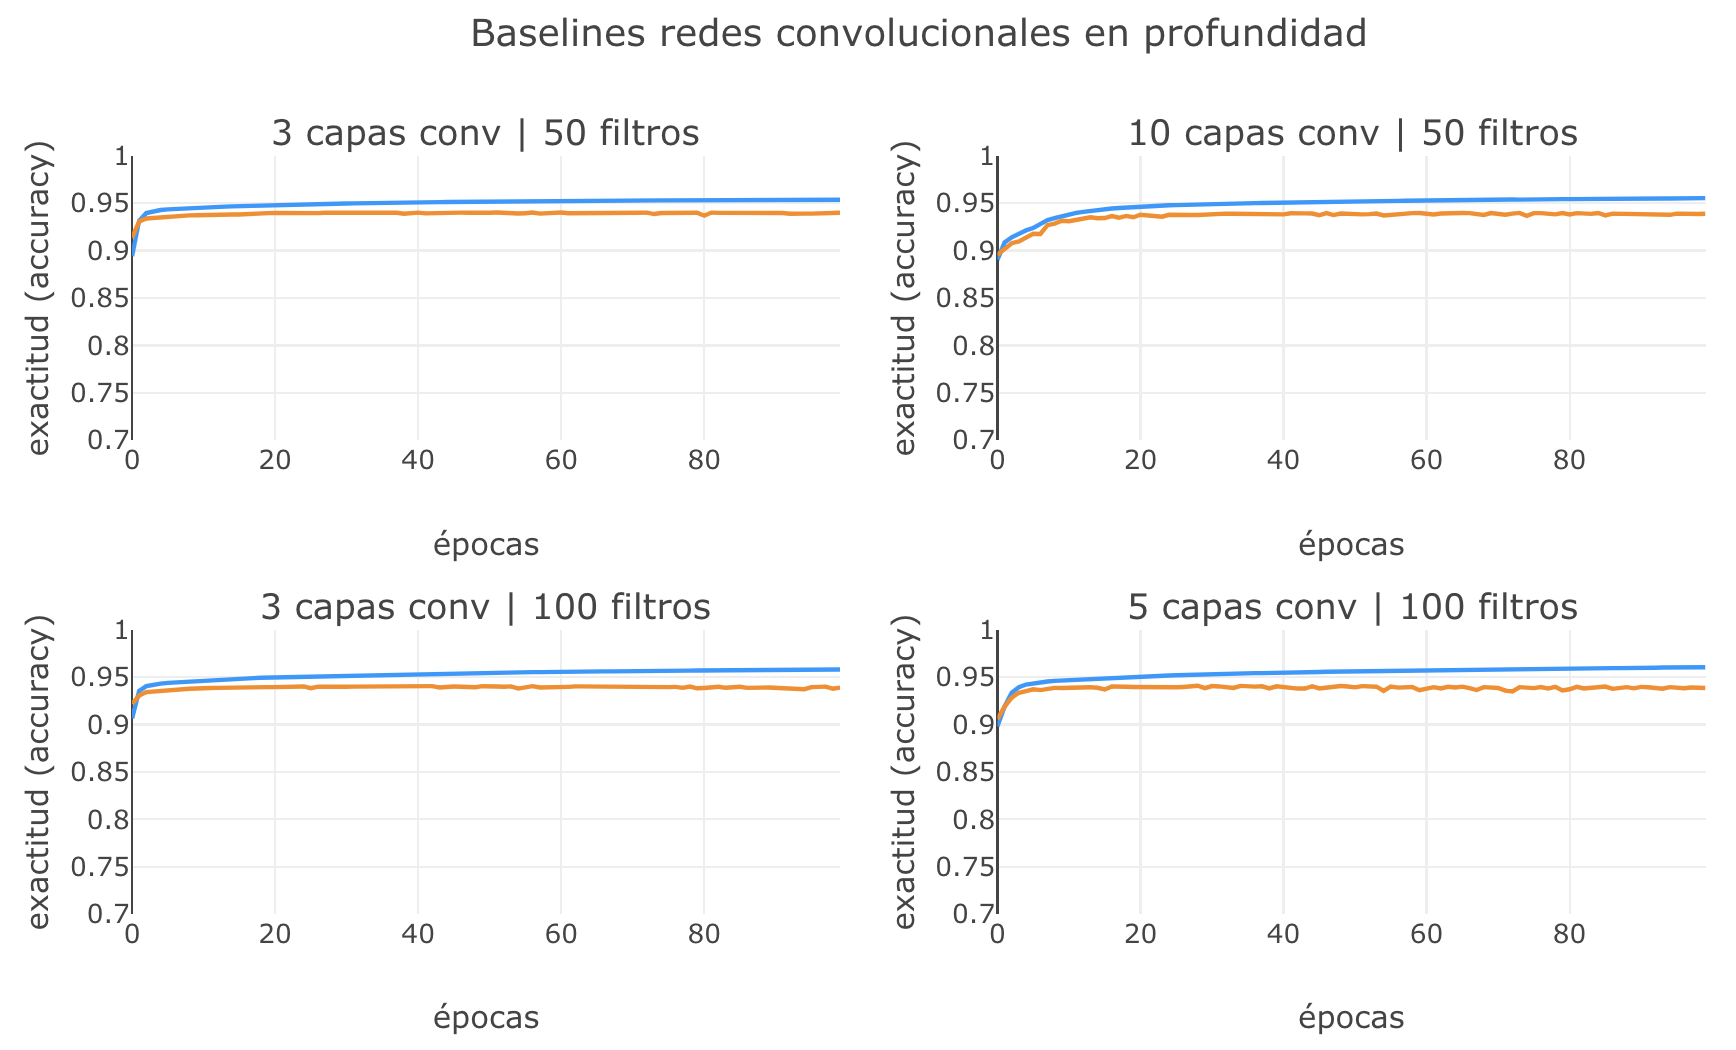
\includegraphics[width=.9\linewidth]{images/CNN_depth_baselines.png}
\caption{Resultado redes convolucionales en profundidad supervisado. Comparación utilizando
distinta cantidad de capas convolucionales y cantidad de filtros por capa.}
\label{fig:CNN_depth_baselines}
\end{center}
\end{figure}

En la Figura \ref{fig:CNN_depth_baselines} se observan cuatro experimentos, los cuales representan los mejores
resultados de los distintos experimentos que se ejecutaron sobre este modelo supervisado. 

Nuevamente el color azul denota el valor de exactitud en los datos de entrenamiento y el anaranjado para el 
caso de los datos de validación. Un aspecto a tener en cuenta es que utilizar como métrica la exactitud para 
su comparación con los modelos anteriores es algo que hay que trabajar con cuidado, ya que al manejar 
instancias a nivel de oración las clases se encuentran inherentemente desbalanceadas, por lo que la exactitud 
puede ser alta simplemente marcando todo como la clase mayoritaria.

Sin embargo, por cuestiones comparativas, sobre todo con los modelos anteriores, se utiliza el experimento 
CNN-Depth-Sup.2 para dicha tarea y con su variante implementación en escalera (en la Figura 
\ref{fig:CNN_depth_baselines}, el de arriba a la derecha, con 10 capas convolucionales y 50 filtros por capa).

\subsection{Comparación de baselines}

Al obtener los mejores hiperparámetros para los modelos baseline, se decidió compararlos para tener una idea 
clara de lo que estamos tratando de lograr superar con la ayuda de las redes en escalera. Para esto, el método
de comparación es con el conjunto de datos de evaluación, en lugar del conjunto de datos de validación.

La Figura \ref{fig:best_supervised_baselines} compara los resultados de los mejores modelos de cada variante 
supervisada. Es un gráfico de barras con agrupación. El eje $y$ del gráfico muestra la exactitud ({\em 
accuracy}) del experimento, donde a mayor valor, mejor el resultado. Por otro lado,
el eje $x$ representa cada uno de los mejores experimentos, 
agrupando tres barras de acuerdo al conjunto de datos sobre el que se muestra el resultado. De esta manera, la
barra azul muestra el resultado sobre el conjunto de entrenamiento y la barra verde sobre el conjunto de 
evaluación ({\em test}).

En la Figura \ref{fig:best_supervised_baselines} se puede observar la notable mejora que aportan los modelos 
basados en redes convolucionales. Se valida el hecho de que aplicar capas convolucionales provoca que se 
capture información del contexto de cada palabra generando buenos atributos ({\em features}) intermedios que 
el modelo utiliza para la tarea de clasificación de entidades nombradas. 

En otras palabras, el uso de capas convolucionales con la finalidad de extraer características del entorno de 
una palabra parece ser una muy buena alternativa.

Por otro lado, se observa que las redes convolucionales en profundidad arrojan los mejores resultado. De todas
maneras, cabe recordar que el uso de exactitud puede esconder el desempeño del modelo para clases 
minoritarias, por lo que hay que tomarlo con cuidado.

\begin{figure}[t]
\begin{center}
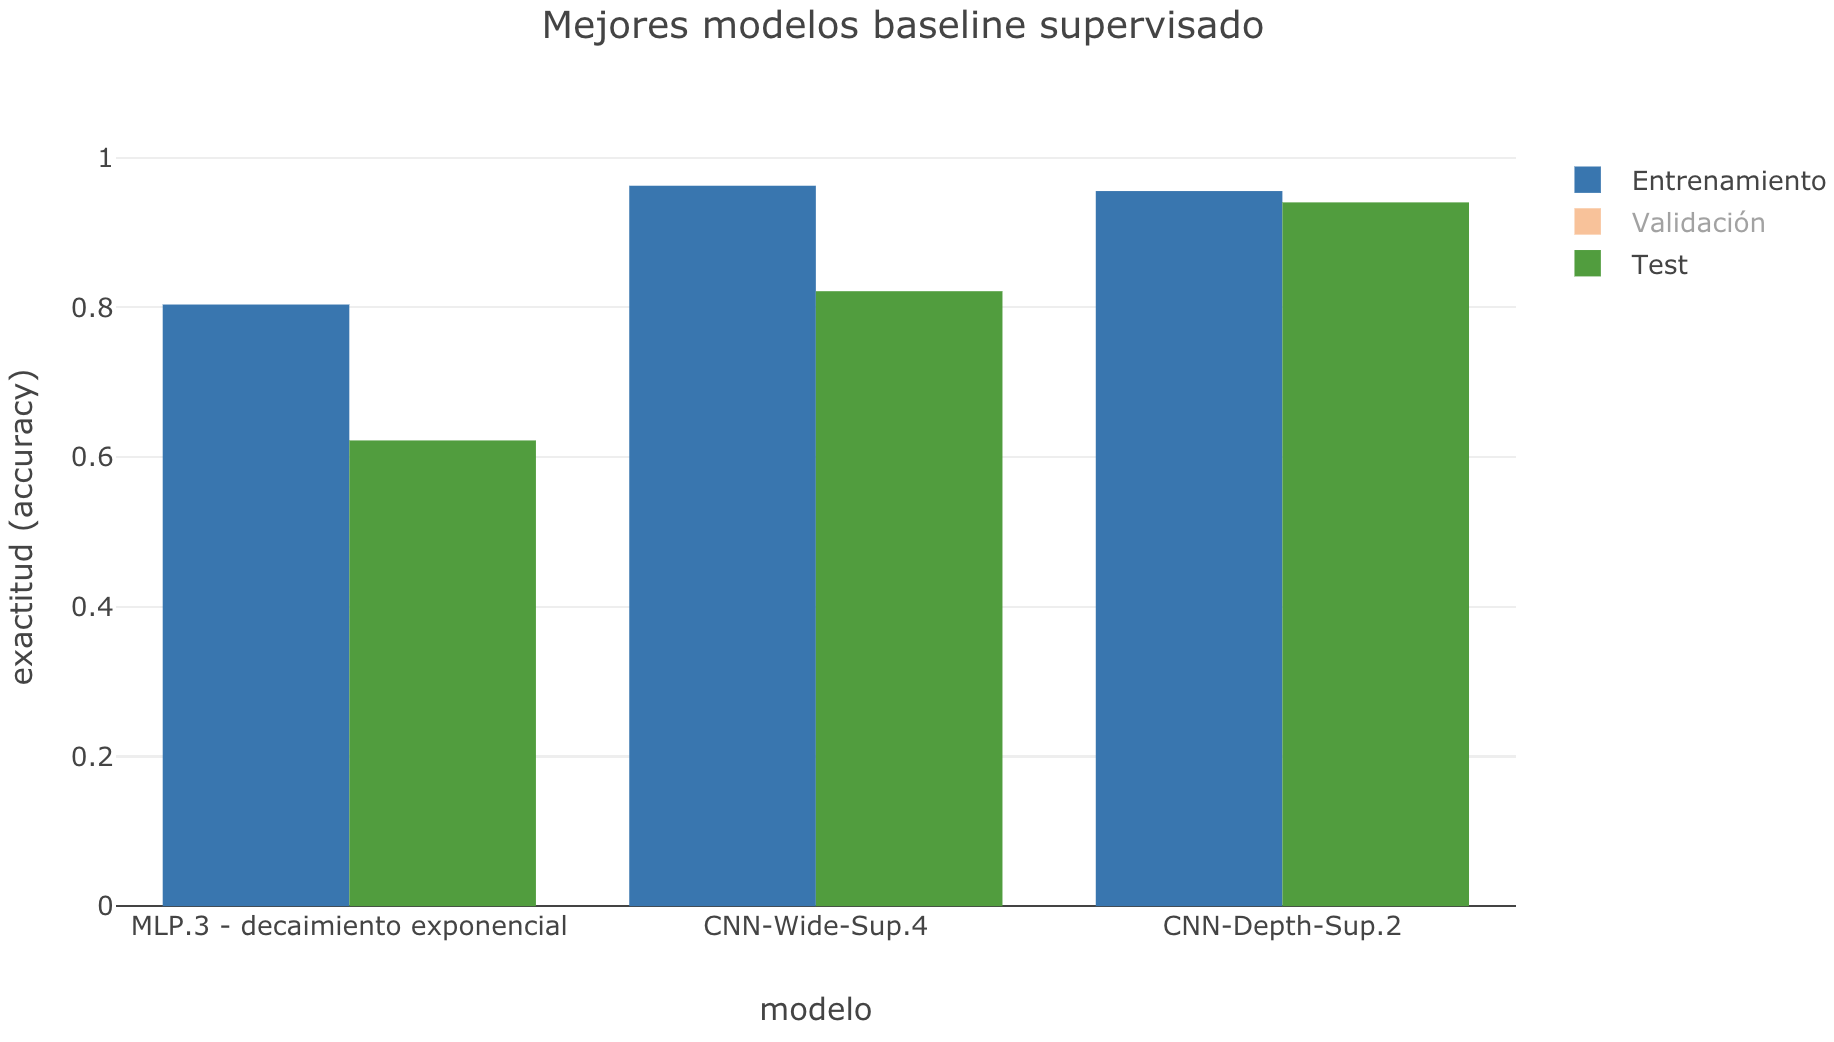
\includegraphics[width=.9\linewidth]{images/best_supervised_baselines.png}
\caption{Mejores modelos baseline supervisados. Comparación de resultados entre datos de entrenamiento y
datos de evaluación}
\label{fig:best_supervised_baselines}
\end{center}
\end{figure}

\section{Redes neuronales en escalera}

Una vez realizados los experimentos netamente supervisados a modo de baseline se prosiguió con la 
incorporación de la tarea no supervisada al utilizar las redes en escalera. Para cada variante se utilizó la 
misma división y conjunto de datos que en los experimentos anteriores, de manera tal que el impacto de los
datos no supervisados pudiese ser medido acorde al experimento realizado.

\subsection{Impacto de los datos no anotados: Perceptrón multicapa en escalera}

En primer lugar, se desea medir el impacto de la tarea no supervisada que brinda la arquitectura en escalera. 
Al incorporar al entrenamiento la utilización de datos no anotados queremos observar si efectivamente derivan 
en una mejora de rendimiento de la red en escalera más básica: el perceptrón multicapa.

Se seleccionó el experimento con mejores resultados del modelo de perceptrón multicapa en escalera para su 
inmediata comparación con su versión supervisada. El Cuadro \ref{tab:exp:mlp_ladder} muestra los 
hiperparámetros de dicho experimento.

\begin{table}[t]
    \centering
    \begin{tabular}{|l|l|l|}
        \hline
        \textbf{Experimento} & \textbf{Hiperparámetro} & \textbf{Valor} \\
        \hline
        \multirow{5}{*}{MLP-Ladder.1} & Representación & Decaimiento exp. \\
                              & Ventana & 5 \\
                              & Capas & [300, 256, 128, 5] \\
                              & Factor de ruido por capa & 0.3 \\
                              & Costo de reducción de ruido & [100, 0.1, 0.1, 0.01] \\
                              & Tasa de aprendizaje & 0.02 \\
        \hline
    \end{tabular}
    \caption{Hiperparámetros del conjunto de experimentos con perceptrón multicapa en escalera.}
    \label{tab:exp:mlp_ladder}
\end{table}

\subsubsection{Evolución de datos de entrenamiento vs. validación a través de épocas}

\begin{figure}[t]
\begin{center}
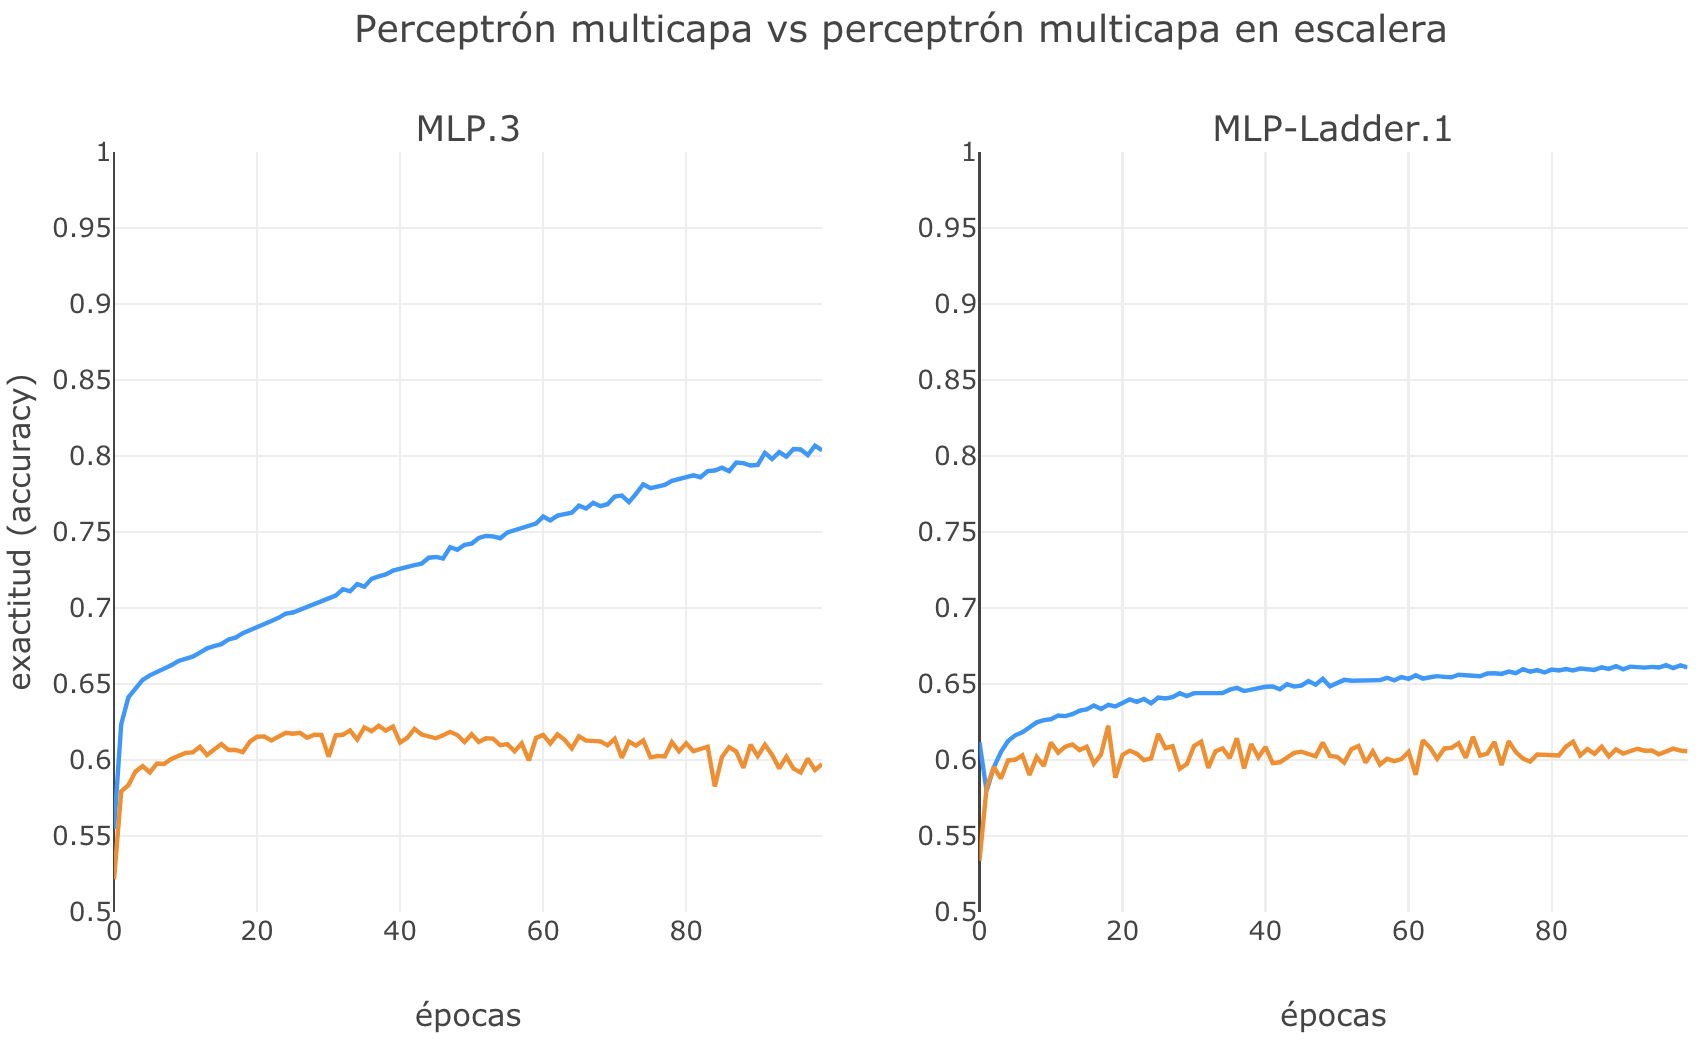
\includegraphics[width=.9\linewidth]{images/MLP_supervised_ladder.png}
\caption{Perceptrón multicapa supervisado vs semisupervisado (escalera). Comparación de evolución de
datos de entrenamiento y datos de validación}
\label{fig:MLP_supervised_ladder}
\end{center}
\end{figure}

En la Figura \ref{fig:MLP_supervised_ladder} se observan dos gráficos, las trazas azules describen el valor de
exactitud del modelo a lo largo de las épocas en los datos de entrenamiento y las trazas anaranjadas de manera
análoga en los datos de validación. El gráfico a izquierda corresponde al experimento MLP.3 que utiliza la 
estrategia de decaimiento exponencial para representar cada palabra y que consiguió el mejor desempeño en la 
Sección \ref{baseline:mlp}. 

Por otro lado, el gráfico a derecha es un experimento equivalente (i.e. con los mismos hiperparámetros y datos
de entrenamiento y validación) en su versión en escalera.

Se puede apreciar como el modelo en escalera permite una mejor generalización que el netamente supervisado al 
observar que la curva correspondiente a los datos de validación acompaña a la de entrenamiento (i.e. el `gap' entre entrenamiento y validación no es tan alto). Más aún, se observa como para el caso del experimento 
puramente supervisado, después de ciertas iteraciones el desempeño sobre validación comienza a caer. En el 
caso del experimento semi-supervisado, por el contrario, el desempeño entre entrenamiento y validación se 
mantiene bastante constante a lo largo del tiempo, lo que es un primer indicio de que el modelo 
semi-supervisado sirve para regularizar el modelo.

\subsubsection{Comparación de valores finales de desempeño sobre datos de entrenamiento vs. evaluación}

La figura \ref{fig:MLP_supervised_ladder_bar} muestra los valores de exactitud para los datos de entrenamiento
y evaluación de los modelos del perceptrón multicapa supervisado y su variante en escalera. 

Es un gráfico de barras con agrupación. El eje $y$ del gráfico muestra la exactitud ({\em accuracy}) del 
experimento, donde a mayor valor, mejor el resultado. Por otro lado, el eje $x$ representa el modelo 
utilizado, agrupando dos barras de acuerdo al conjunto de datos sobre el que se muestra el resultado. 

De esta manera, la barra azul muestra el resultado sobre el conjunto de entrenamiento y la barra verde sobre 
el conjunto de evaluación ({\em test}). Nuevamente se observa una mayor generalización por parte del modelo 
perceptrón multicapa en escalera ({\em MLP-Ladder.1}) ya que la diferencia en cuanto al desempeño en los datos
de evaluación y entrenamiento es notablemente menor, mientras que el desempeño en el conjunto de datos de 
evaluación para el método semi-supervisado es igual (sino mayor) al mostrado para el caso puramente 
supervisado. Junto con los resultados de la Figura \ref{fig:MLP_supervised_ladder}, podemos concluir que
el uso de datos no anotados en el modelo arroja resultados interesantes a la hora de regularizar dicho
modelo.

\begin{figure}[t]
\begin{center}
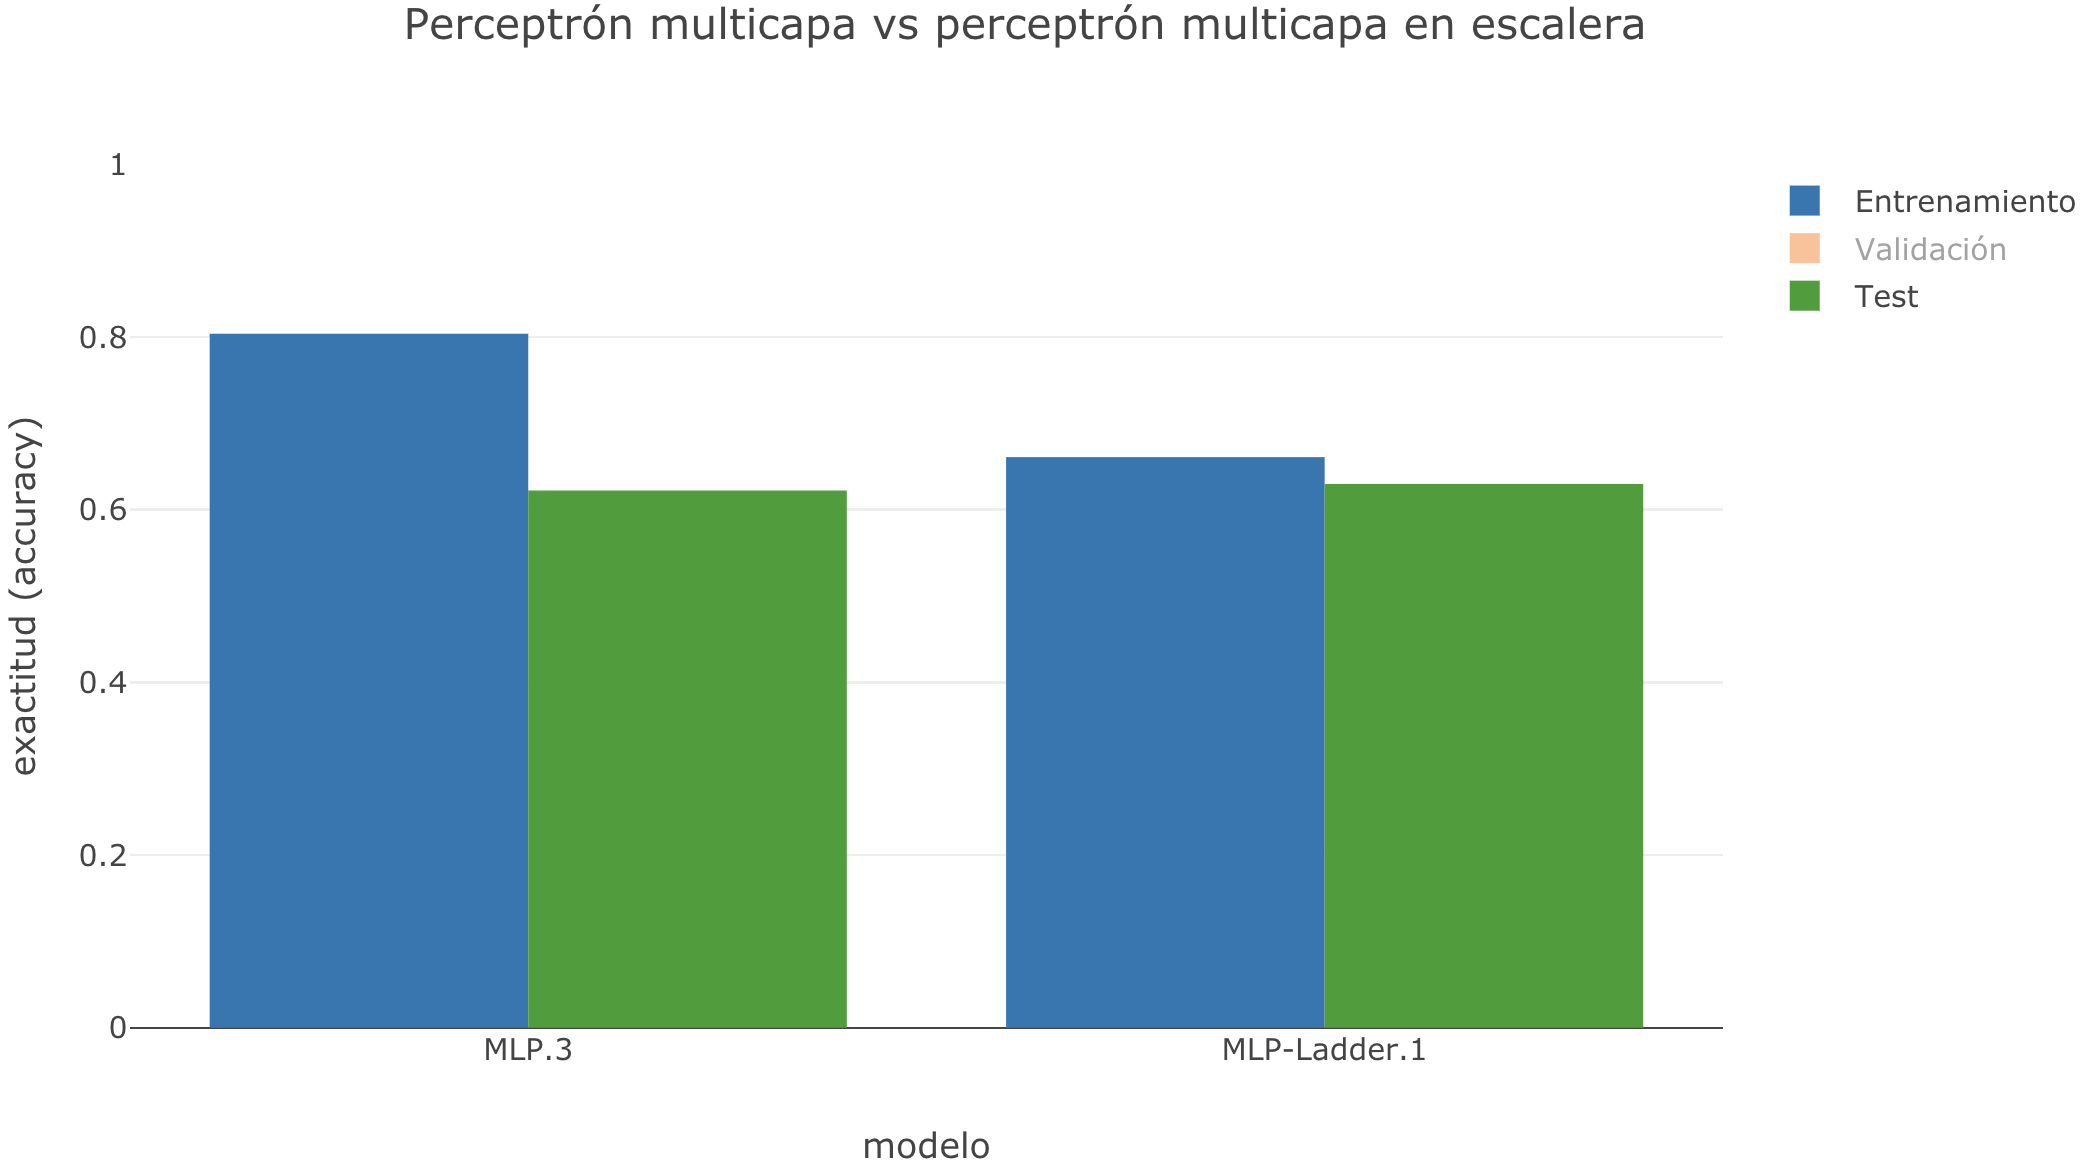
\includegraphics[width=.9\linewidth]{images/MLP_supervised_ladder_bar.png}
\caption{Perceptrón multicapa supervisado vs semisupervisado (escalera). Comparación de resultados finales
sobre datos de entrenamiento y datos de validación}
\label{fig:MLP_supervised_ladder_bar}
\end{center}
\end{figure}

\subsection{Impacto de selección de datos anotados y no anotados para el entrenamiento: Redes convolucionales 
en escalera en amplitud}

Este conjunto de experimentos busca medir el impacto de utilizar distintos tipos de datos de entrenamiento
para los modelos semi-supervisados de redes en escalera. En particular, nos interesa observar como se comporta
un modelo de red en escalera convolucional en amplitud a partir de la que se define en la Sección 
\ref{sec:cnn:wide}. 

Se observan distintas combinaciones de datos anotados y no anotados como entrenamiento para los modelos de la 
red convolucional en escalera. No obstante, se mantienen las mismas 20000 instancias de validación y 20000 de 
evaluación utilizadas en la versión supervisada para poder comparar con el baseline supervisado de la Sección 
\ref{baseline:cnn:wide}.

\begin{table}[b!]
    \centering
    \begin{tabular}{|l|l|l|}
        \hline
        \textbf{Experimento} & \textbf{Hiperparámetro} & \textbf{Valor} \\
        \hline
        \multirow{8}{*}{Hiper. generales} & Ventana simétrica W & 2 \\
                              & Número de filtros & 100 \\
                              & Factor de ruido por capa & 0.3 \\
                              & Costo de reducción de ruido & [100, 0.1, 0.01] \\
                              & Factor costo no supervisado & 0.3 \\
                              & Tasa de aprendizaje & 0.02 \\
                              & Tamaño de max pooling & 1 \\
                              & Tamaño de kernels & [2,3,4] \\
                              
        \hline
        \multirow{2}{*}{CNN-Wide-Ladder.1} & Datos anotados & 100k \\
                                           & Datos no anotados & mismos 100k \\
        \hline
        \multirow{2}{*}{CNN-Wide-Ladder.2} & Datos anotados & 100k \\
                                           & Datos no anotados & 100k disjuntos \\
        \hline
        \multirow{2}{*}{CNN-Wide-Ladder.3} & Datos anotados & 100k \\
                                           & Datos no anotados & 200k \\
        \hline
    \end{tabular}
    \caption{Hiperparámetros del conjunto de experimentos con redes convolucionales en amplitud en escalera.}
    \label{tab:exp:cnn_wide_ladder}
\end{table}

Notar que en estos casos, a diferencia del perceptrón multicapa de la sección anterior, un ejemplo de 
entrenamiento es un fragmento de oración como se detalla en la Sección \ref{sec:fragmento_sentencia}. 

El Cuadro \ref{tab:exp:cnn_wide_ladder} detalla los experimentos realizados con las redes convolucionales
en escalera en amplitud, basadas en lo detallado en la Sección \ref{sec:cnn:wide}.

Para el caso del modelo de redes convolucionales en amplitud en escalera se muestran tres experimentos, con 
los hiperparámetros generales que mejores resultados obtuvieron seleccionados de manera aleatoria. 

Lo que varían en estos experimentos son las instancias utilizadas para el entrenamiento del modelo, la razón 
de esto es medir el impacto que generan los datos no anotados dependiendo si coinciden o no con los anotados y
que sucede si variamos la proporción utilizada.

\subsubsection{Comparación de distintos tipos de datos de entrada: iguales, disjuntos y contenidos}

\begin{figure}[t]
\begin{center}
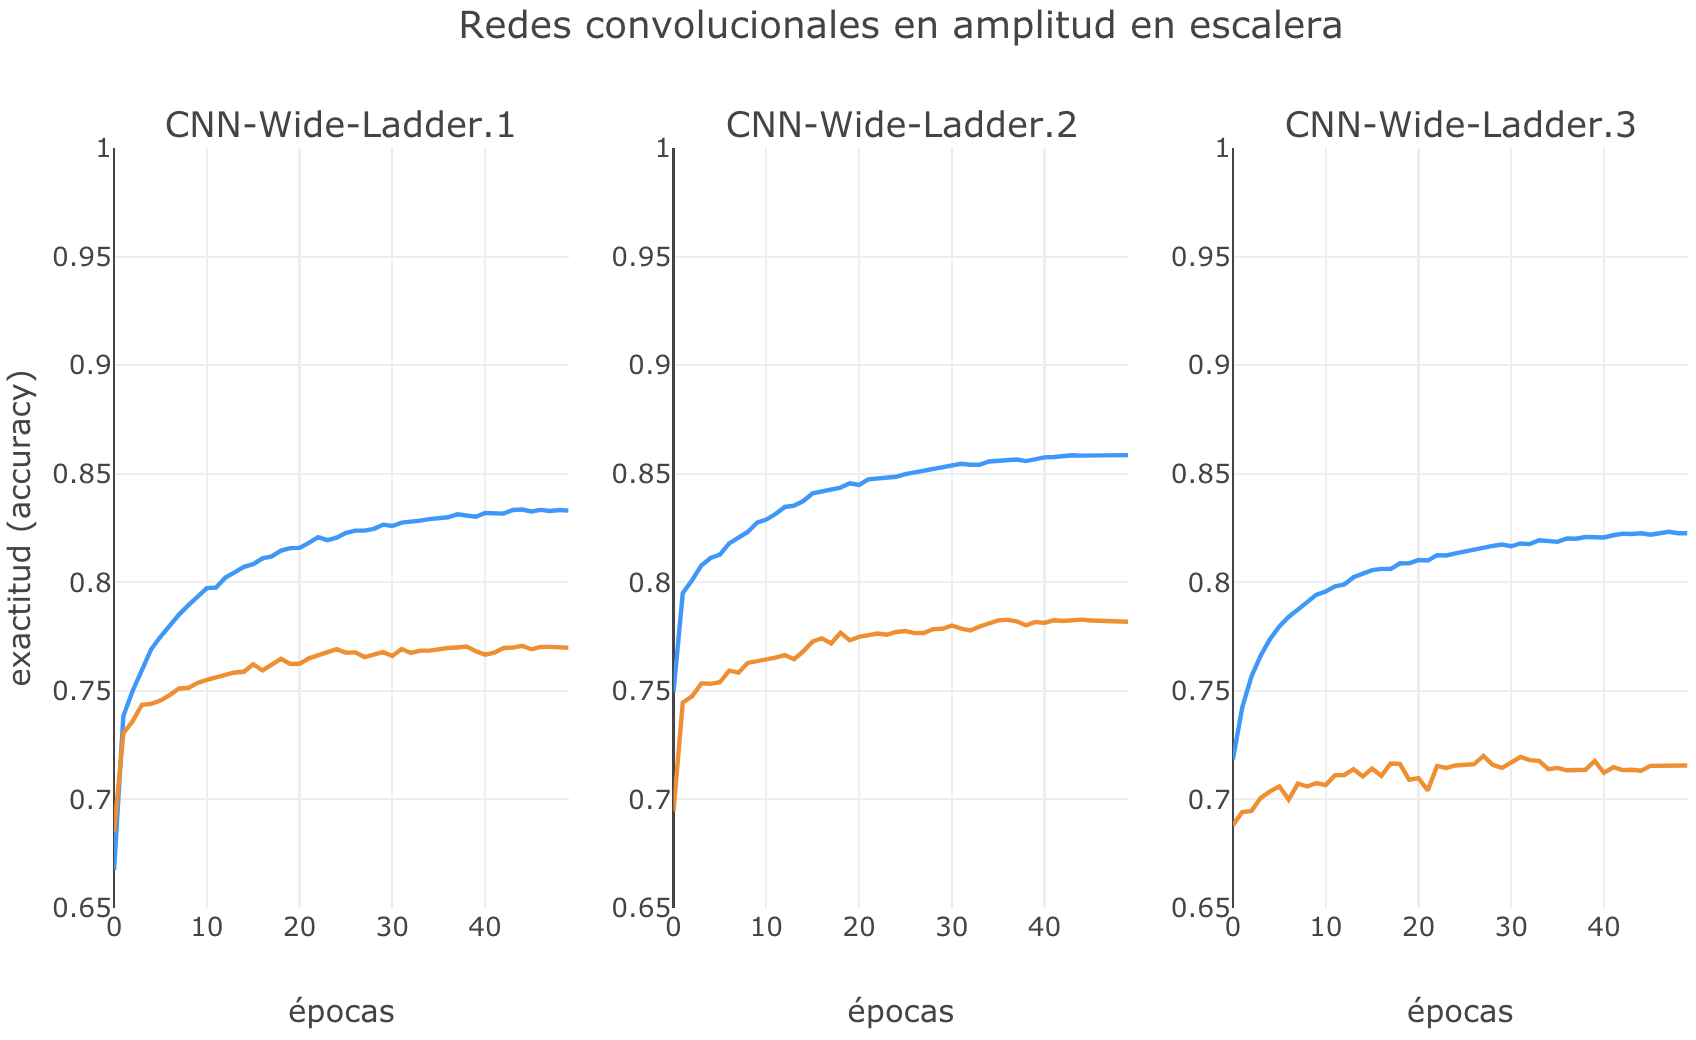
\includegraphics[width=.9\linewidth]{images/CNN_wide_ladder.png}
\caption{Redes convolucionales en amplitud en escalera. Comparación de resultados utilizando distintos
conjuntos de entrenamiento anotado y no anotado.}
\label{fig:CNN_wide_ladder}
\end{center}
\end{figure}

En la figura \ref{fig:CNN_wide_ladder} se observan tres gráficos correspondientes a los experimentos 
realizados sobre el modelo de redes convolucionales en amplitud en escalera. 

A izquierda se ubica el gráfico correspondiente a utilizar las mismas 100k instancias de entrenamiento como 
datos anotados y no anotados. 

El gráfico central es el resultante de haber utilizado 100k instancias anotadas y 100k instancias disjuntas no anotadas. 

Por último, el gráfico de la derecha utiliza las 100k instancias originales como datos anotados y no anotados 
y, a su vez, suma 100k nuevos no anotados. 

El experimento CNN-Wide-Ladder.2 nos muestra que agregar nuevos datos no anotados parece ser clave para 
mejorar el rendimiento del modelo. Sin embargo agregar demasiados datos no anotados puede afectar al modelo de
manera negativa como se observa en el experimento CNN-Wide-Ladder.3. Esto último puede deberse al hecho de que
la red no es lo suficientemente capaz de manejar la reconstrucción de tantos datos no anotados, quizás se 
requeriría una red de mayor tamaño para dicha tarea.

\subsubsection{Comparación de resultados supervisados y semi-supervisados en la evolución de entrenamiento vs.
validación por épocas}

La Figura \ref{fig:CNN_wide_supervised_ladder} hace una comparación del mejor modelo obtenido en
la Sección \ref{baseline:cnn:wide} y el modelo obtenido con CNN-Wide-Ladder.2. 

\begin{figure}[t]
\begin{center}
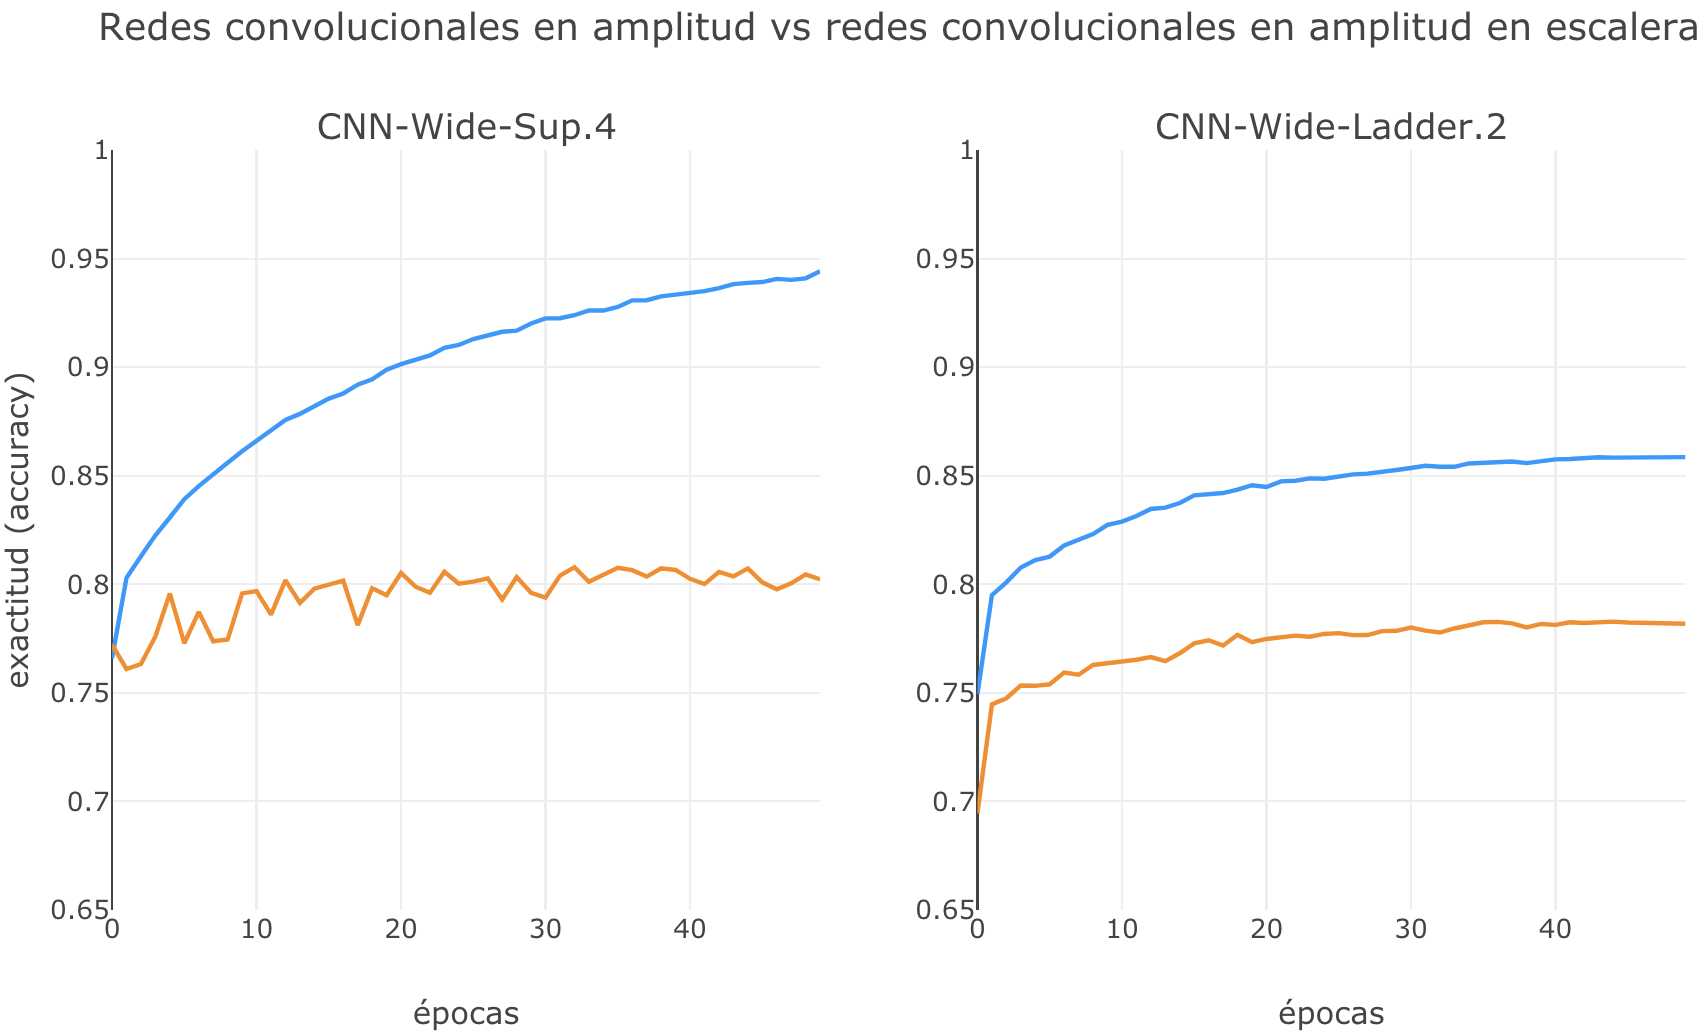
\includegraphics[width=.9\linewidth]{images/CNN_wide_supervised_ladder.png}
\caption{Modelo de redes convolucionales en amplitud supervisado vs semi-supervisado (escalera). Comparación
de evolución en épocas del desempeño en corpus de entrenamiento y corpus de validación.}
\label{fig:CNN_wide_supervised_ladder}
\end{center}
\end{figure}

Como se puede observar, la implementación del modelo de redes convolucionales en amplitud en escalera, la 
curva anaranjada (validación) acompaña a una distancia más cercana a la curva azul (entrenamiento) que en el 
caso del modelo supervisado. 

Más aún, si bien en este caso el desempeño del modelo semisupervisado sobre el conjunto de datos de validación
es ligeramente menor que para el modelo puramente supervisado (medido mediante la exactitud), se muestra menor
ruido en el desempeño.

De manera análoga al modelo perceptrón multicapa en escalera, se comprueba que la tarea no supervisada 
colabora en la generalización del modelo.

\subsubsection{Comparación de precisión y exhaustividad por clase supervisados y semi-supervisados con 
resultados sobre datos de evaluación}

Finalmente, para una comparación más detallada, con métricas de precisión y exhaustividad ({\em precisión \& 
recall}), la Figura \ref{fig:CNN_wide_supervised_ladder_precision_recall} presenta una comparación clase por 
clase entre los dos modelos para el conjunto de datos de evaluación. En el gráfico, cada cuarto representa la 
clase a comparar (PER, LOC, ORG, y MISC, la clase O no se compara). Es un gráfico de barras agrupadas de 
acuerdo al modelo (redes convolucionales en amplitud supervisadas y no supervisadas).

La barra de color rojo representa el valor de exhaustividad que obtuvo cada modelo para cada clase en 
particular sobre el conjunto de datos de evaluación. La barra de color color ocre representa los valores de 
precisión obtenidos. No se observan grandes diferencias entre los modelos, con el modelo supervisado superando
en algunos casos al semi-supervisado y viceversa. Posteriormente se utilizarán estos resultados para su 
comparación con el modelo de redes convolucionales en profundidad.

\begin{figure}[h]
\begin{center}
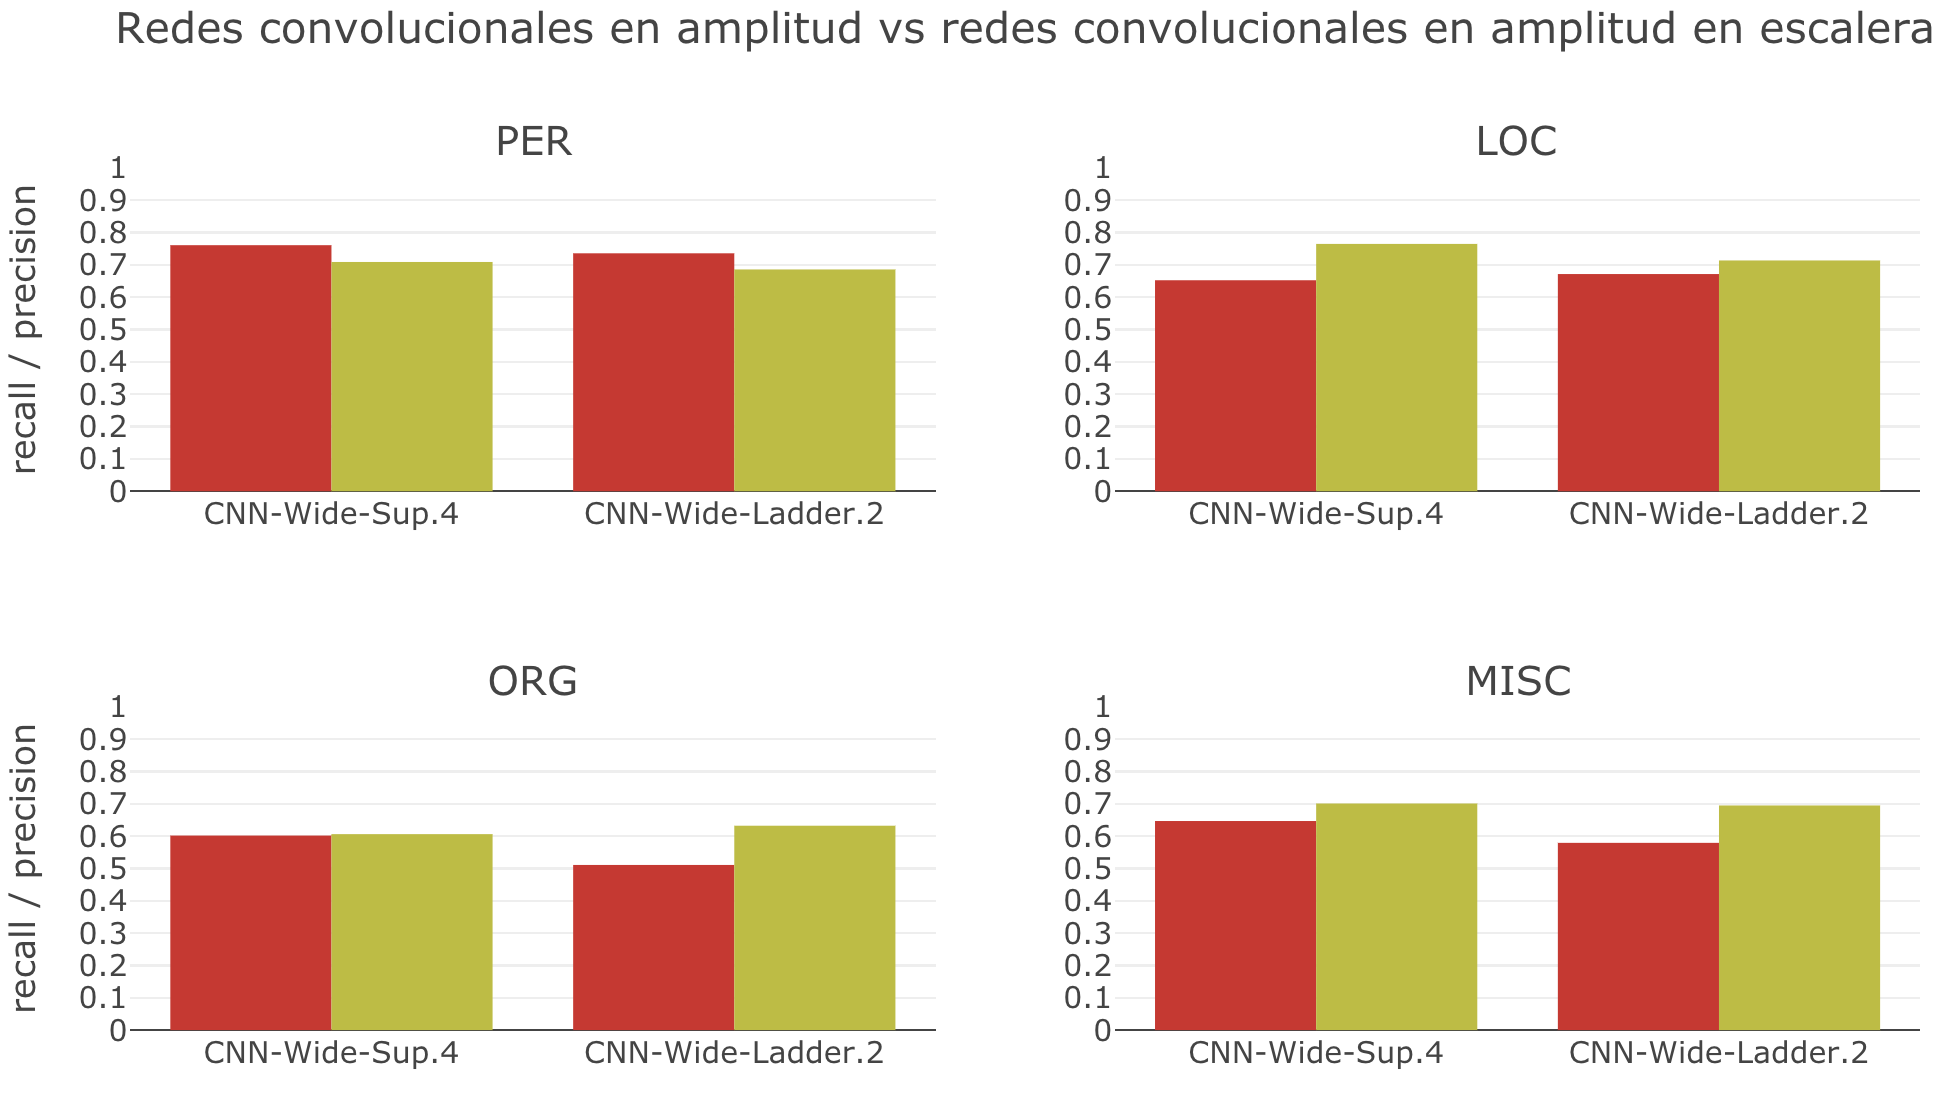
\includegraphics[width=.9\linewidth]{images/CNN_wide_supervised_ladder_precision_recall.png}
\caption{Modelo de redes convolucionales en amplitud supervisado vs semi-supervisado (escalera). Comparación
de desempeño mediante precisión y exhaustividad por clase sobre conjunto de datos de evaluación.}
\label{fig:CNN_wide_supervised_ladder_precision_recall}
\end{center}
\end{figure}

\subsection{Impacto de datos anotados para entrenamiento: Redes convolucionales
en escalera en profundidad}

En esta serie de experimentos buscamos medir el impacto del desempeño del modelo modificando la cantidad
inicial de datos anotados sobre los cuales entrenar la parte supervisada del modelo. 

Como caso de estudio, se utilizaron las redes convolucionales en escalera en profundidad definidas en la 
Sección \ref{sec:cnn:deep}, ya que en estas el desempeño de la parte supervisada del modelo era esencial 
puesto que no se pueden, por la naturaleza de los datos secuenciales, subsamplear la clase mayoritarias ``O''.
Por lo que queremos ver efectivamente que tan importante es el uso de datos anotados para el desempeño general
del modelo semi-supervisado.

\begin{table}[b!]
    \centering
    \begin{tabular}{|l|l|l|}
        \hline
        \textbf{Experimento} & \textbf{Hiperparámetro} & \textbf{Valor} \\
        \hline
        \multirow{10}{*}{Hiper. generales} & Número de filtros & 100 \\
                              & Capas convolucionales & 10 \\
                              & Factor de ruido por capa & 0.3 \\
                              & Costo ruido capa de entrada & 100 \\
                              & Costo ruido capa convolucional & 0.1 \\
                              & Costo ruido capa de salida & 0.01 \\
                              & Factor costo no supervisado & 0.1 \\
                              & Tasa de aprendizaje & 0.02 \\
                              & Tamaño de kernels & 2 \\
                              & Datos entrenamiento no anotados & 100k \\
                              
        \hline
        \multirow{1}{*}{CNN-Depth-Ladder-a} & Datos entrenamiento anotados & 25k \\
        \hline
        \multirow{1}{*}{CNN-Depth-Ladder-b} & Datos entrenamiento anotados & 50k \\
        \hline
        \multirow{1}{*}{CNN-Depth-Ladder-c} & Datos entrenamiento anotados & 75k \\
        \hline
        \multirow{1}{*}{CNN-Depth-Ladder-d} & Datos entrenamiento anotados & 100k \\
        \hline
    \end{tabular}
    \caption{Hiperparámetros del conjunto de experimentos con redes convolucionales en profundidad en escalera.}
    \label{tab:exp:cnn_depth_ladder}
\end{table}

En los experimentos se varía la proporción de datos anotados en la etapa de entrenamiento con la 
promesa de que el modelo semi-supervisado puede suplir la falta de datos anotados gracias al uso de datos no 
anotados. En estos experimentos, al utilizarse un modelo de etiquetado de secuencias, se evalúan datos
del tipo ``Oración - Etiquetas'' como se definen en la Sección \ref{sec:sequence_labeling}. Notar que este experimento también se realizó en otras arquitecturas en escalera con resultados similares pero con fines de no ser reiterativos se decidió mostrar los resultados para esta arquitectura en particular.

En el Cuadro \ref{tab:exp:cnn_depth_ladder}, se detallan los cuatro experimentos realizados, con los 
hiperparámetros generales que mejores resultados obtuvieron seleccionados de manera aleatoria. Lo que varía 
son las instancias anotadas utilizadas para el entrenamiento del modelo. No obstante, se decidió mostrar únicamente la comparación entre los modelos CNN-Depth-Ladder-a y CNN-Depth-Ladder-d que mostraban los resultados mas relevantes en cuanto a la validación de la hipótesis propuesta.

\subsubsection{Comparación de resultados semi-supervisados al variar la proporción de datos anotados para el entrenamiento.}

En la Figura \ref{fig:CNN_depth_ladder_precision_recall} se observan los valores de \textit{recall} (en color rojo) y de \textit{precision} (en color verde claro) para cada una de las clases que representan una entidad nombrada sobre el conjunto de evaluación. Se compara el modelo de redes convolucionales en profundidad en escalera utilizando 25000 instancias etiquetadas (CNN-Depth-Ladder-a) contra utilizar 100000 instancias etiquetadas (CNN-Depth-Ladder-d) para el entrenamiento del modelo. En general, se obtiene entre 1 y 2 puntos de mejora al utilizar la totalidad de ejemplos etiquetados salvo para los casos de \textit{precision} en la clase PER y de \textit{recall} en la clase MISC donde incluso tomar una proporción menor (25\%) del total de instancias de entrenamiento generó mejores resultados. Vemos entonces la ventaja de trabajar con este modelo semi-supervisado donde tomar una proporción significativamente menor de datos para el entrenamiento no se corresponde con una gran pérdida de desempeño.

\begin{figure}[H]
\begin{center}
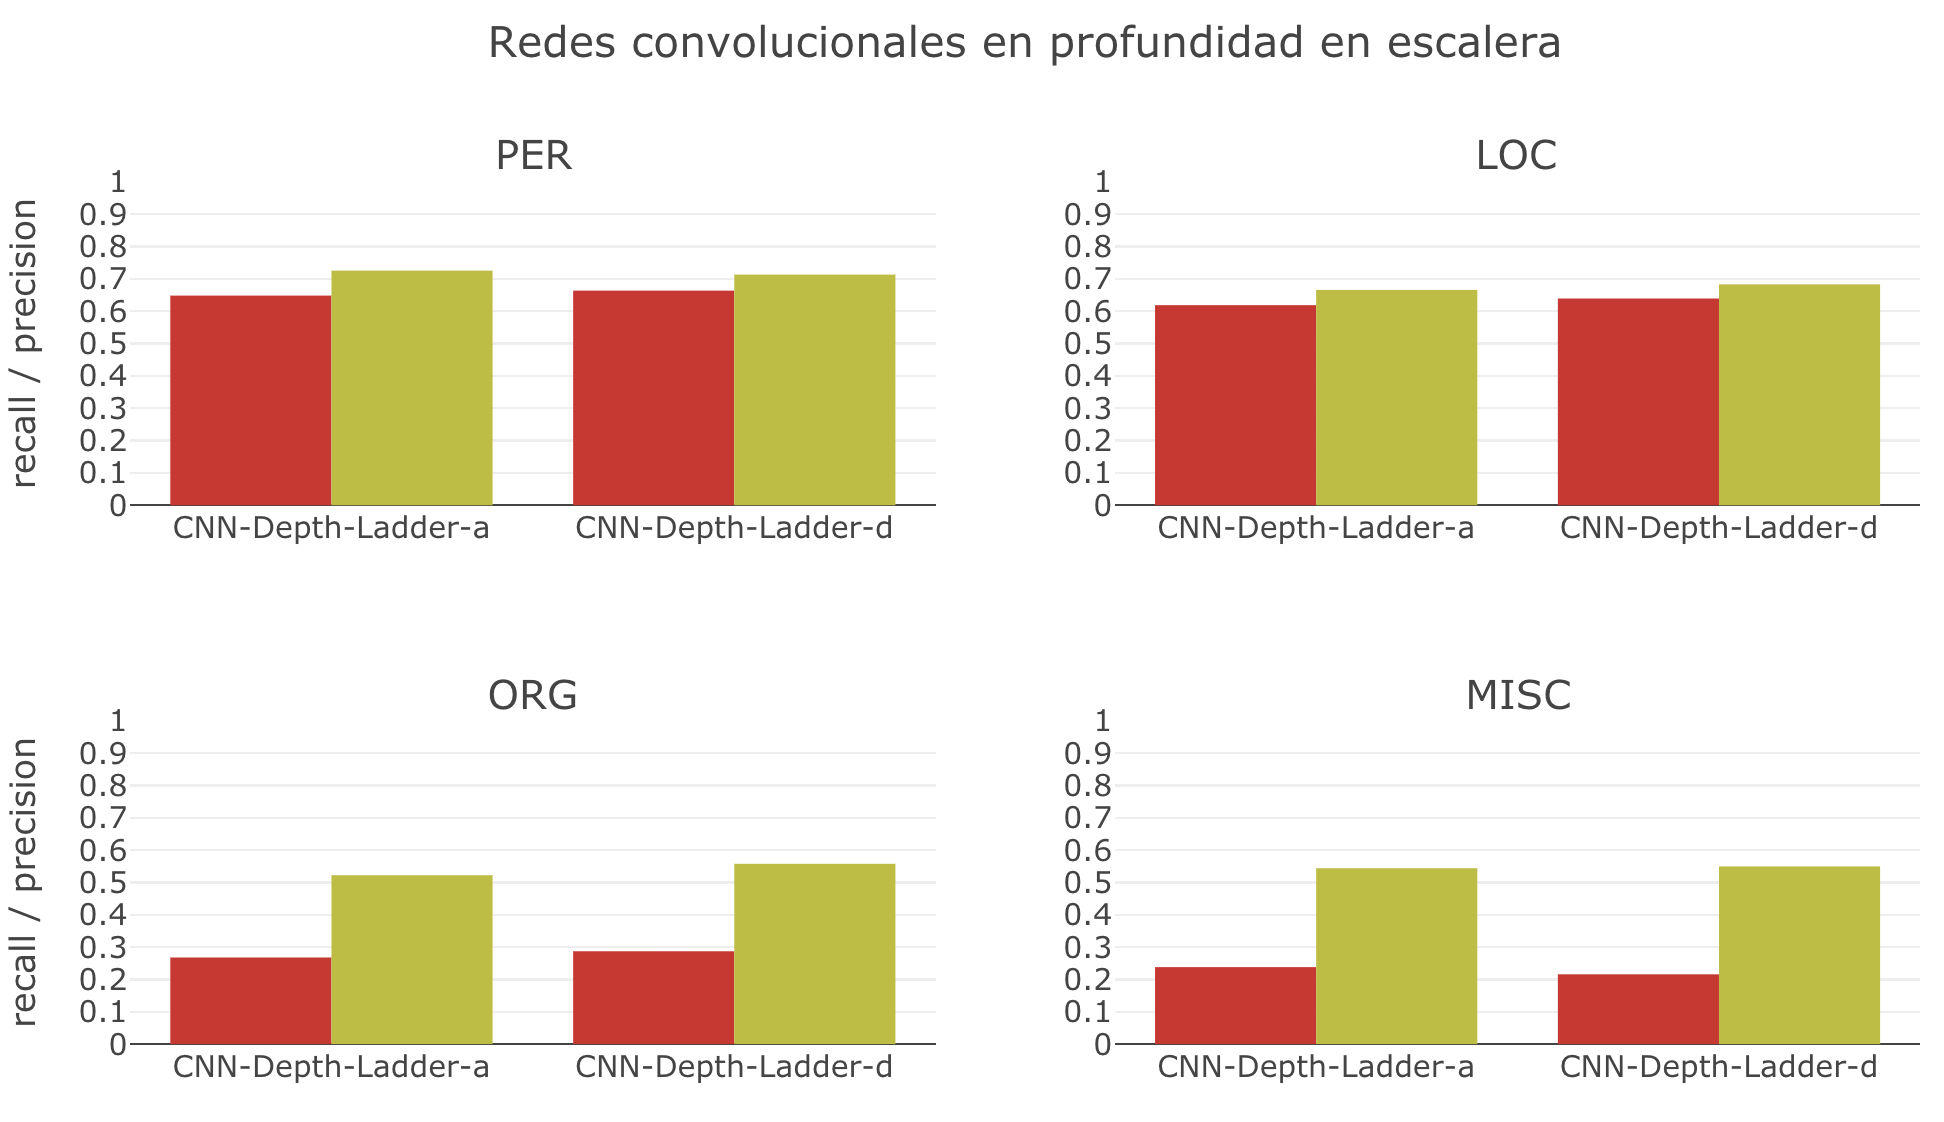
\includegraphics[width=.9\linewidth]{images/CNN_depth_ladder_precision_recall.png}
\caption{Redes convolucionales en profundidad en escalera.}
\label{fig:CNN_depth_ladder_precision_recall}
\end{center}
\end{figure}

\subsubsection{Comparación de mejores resultados de los modelos de redes convolucionales en amplitud y profundidad en escalera.}

En la Figura \ref{fig:CNN_wide_depth_ladder_precision_recall} se comparan los mejores resultados de los modelos de redes convolucionales en amplitud y en profundidad ambos en su variante en escalera. El color rojo se utiliza para los valores de \textit{recall} y el verde claro para los valores de \textit{precision} alcanzados por cada uno de los modelos en sus correspondientes conjuntos de evaluación. El modelo de redes convolucionales posee un desempeño superior visible en todas las clases y de manera más notable en las categorías ORG y MISC, sólo en el caso de \textit{precision} para la categoria PER el modelo de redes convolucionales en profundidad es ligeramente superior.

\begin{figure}[H]
\begin{center}
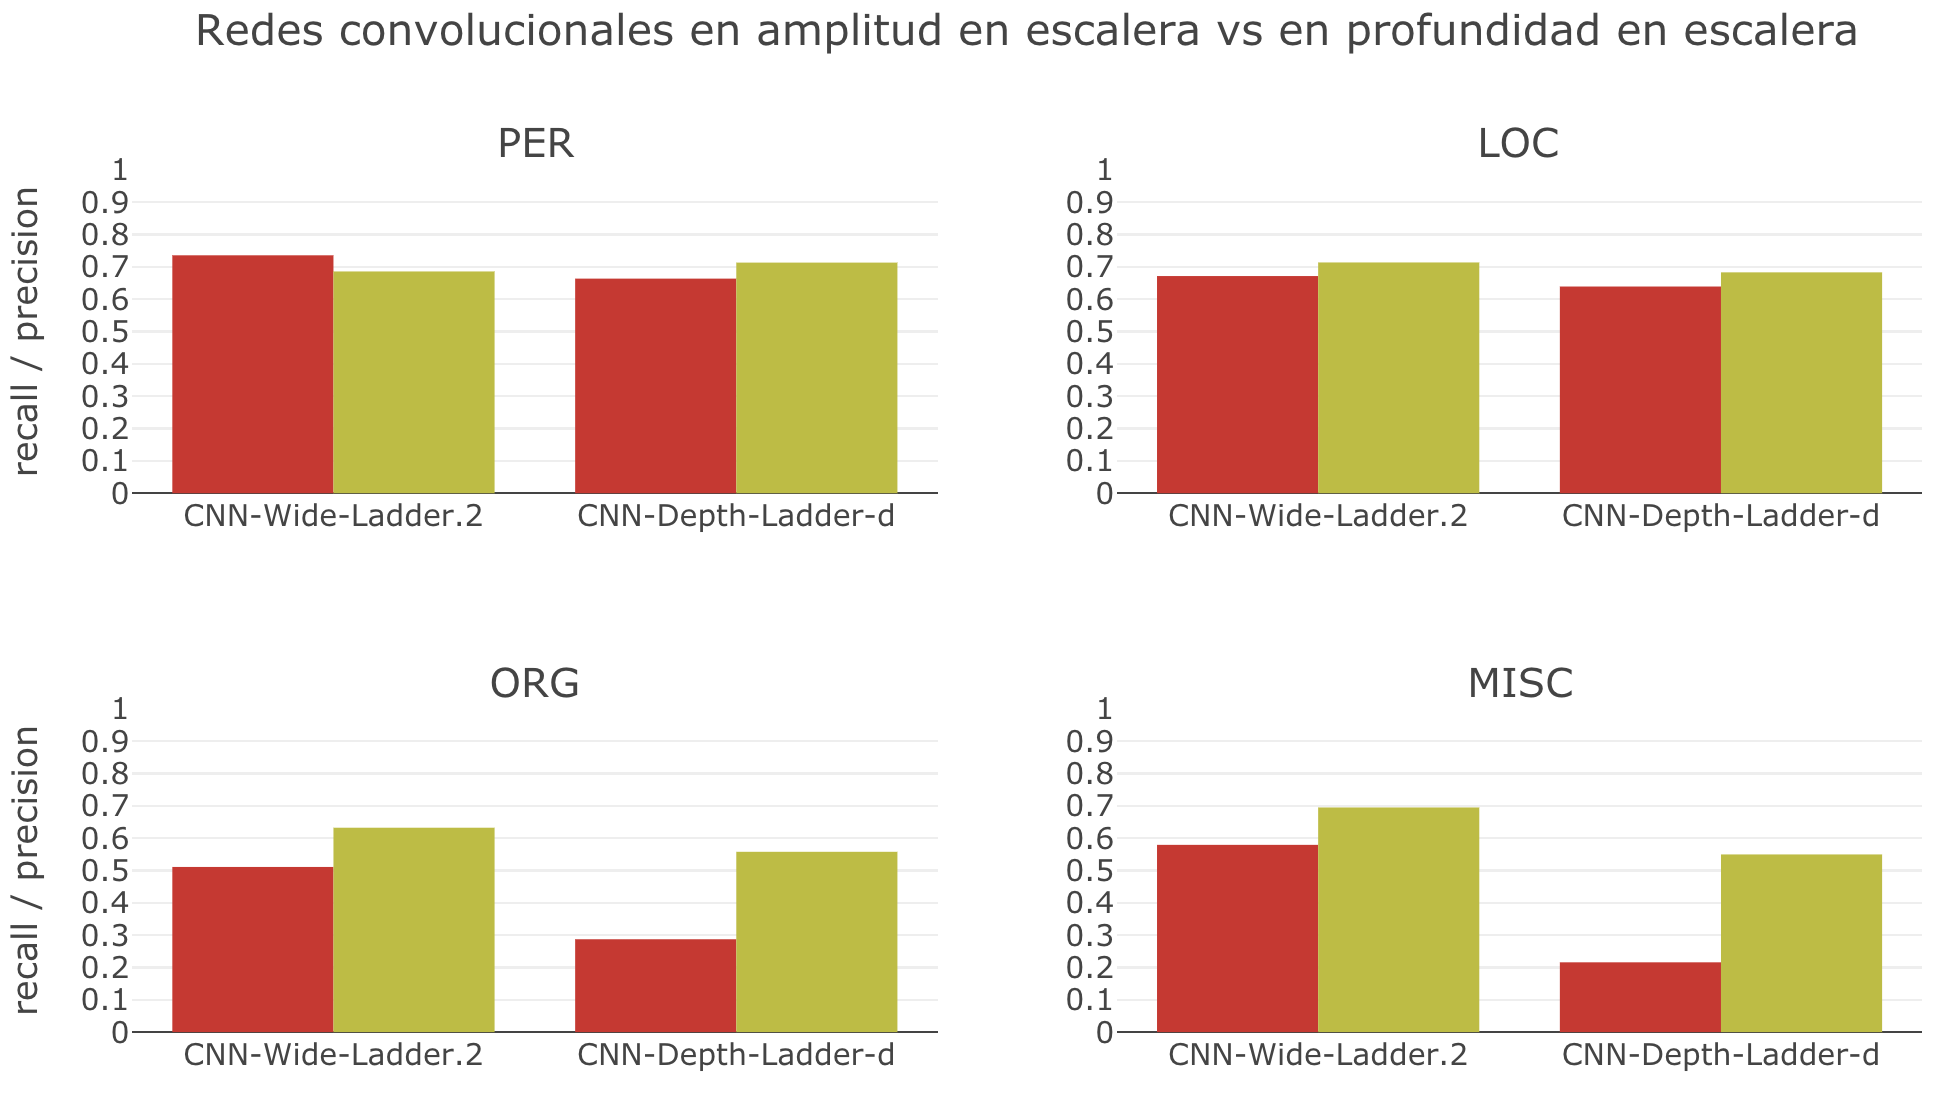
\includegraphics[width=.9\linewidth]{images/CNN_wide_depth_ladder_precision_recall.png}
\caption{Redes convolucionales en amplitud en escalera vs en profundidad en escalera.}
\label{fig:CNN_wide_depth_ladder_precision_recall}
\end{center}
\end{figure}

\subsection{Impacto del costo no supervisado en el aprendizaje del modelo: Redes convolucionales en escalera en profundidad}

Una hipótesis que surgió a lo largo de este trabajo fue si brindar demasiada importancia a la tarea no supervisada perjudica el entrenamiento del modelo ya que el mismo se concentraría en la reconstrucción de la entrada en lugar de la tarea prioritaria de predicción. Para ello, se agregó un factor $\mu$ detallado en \ref{sec:ladder_net} que nos permitiera ajustar el peso del costo no supervisado. 

\begin{table}[H]%[b!]
    \centering
    \begin{tabular}{|l|l|l|}
        \hline
        \textbf{Experimento} & \textbf{Hiperparámetro} & \textbf{Valor} \\
        \hline
        \multirow{10}{*}{Hiper. generales} & Número de filtros & 100 \\
                              & Capas convolucionales & 10 \\
                              & Factor de ruido por capa & 0.3 \\
                              & Costo ruido capa de entrada & 100 \\
                              & Costo ruido capa convolucional & 0.1 \\
                              & Costo ruido capa de salida & 0.01 \\
                              & Factor costo no supervisado & 0.1 \\
                              & Tasa de aprendizaje & 0.02 \\
                              & Tamaño de kernels & 2 \\
                              & Datos entrenamiento no anotados & 100k \\
                              
        \hline
        \multirow{1}{*}{u\_cost 0} & Valor de \mu & 0 \\
        \hline
        \multirow{1}{*}{u\_cost 0.1} & Valor de \mu & 0.1 \\
        \hline
        \multirow{1}{*}{u\_cost 0.3} & Valor de \mu & 0.3 \\
        \hline
        \multirow{1}{*}{u\_cost 0.5} & Valor de \mu & 0.5 \\
        \hline
    \end{tabular}
    \caption{Hiperparámetros del conjunto de experimentos con redes convolucionales en profundidad en escalera.}
    \label{tab:exp:cnn_depth_ladder_loss}
\end{table}

\subsubsection{Comparación de las curvas de loss durante el entrenamiento del modelo.}

En la Figura \ref{fig:CNN_depth_ladder_loss} se observan los resultados de cuatro experimentos realizados sobre el modelo de redes convolucionales en profundidad en escalera. El valor u\_cost es un factor multiplicativo aplicado a la función de costo no supervisada del modelo (denotado como $\mu$ en la sección \ref{sec:ladder_net}). Por lo cual, a mayor u\_cost mayor es la ponderación que se le da a la función de costo no supervisada que el modelo debe minimizar conjuntamente con la supervisada. El color azul representa el valor de pérdida (\textit{loss}) supervisado del modelo a lo largo de las épocas sobre el conjunto de entrenamiento mientras que el anaranjado sobre el conjunto de validación. Es importante tener en consideración no darle demasiado peso a la función de costo no supervisada, ya que provoca que el modelo se centre demasiado en la tarea de reconstrucción dejando de lado la tarea supervisada de clasificación. Se observa como con un u\_cost de 0.5 ya el modelo diverge.

\begin{figure}[t]
\begin{center}
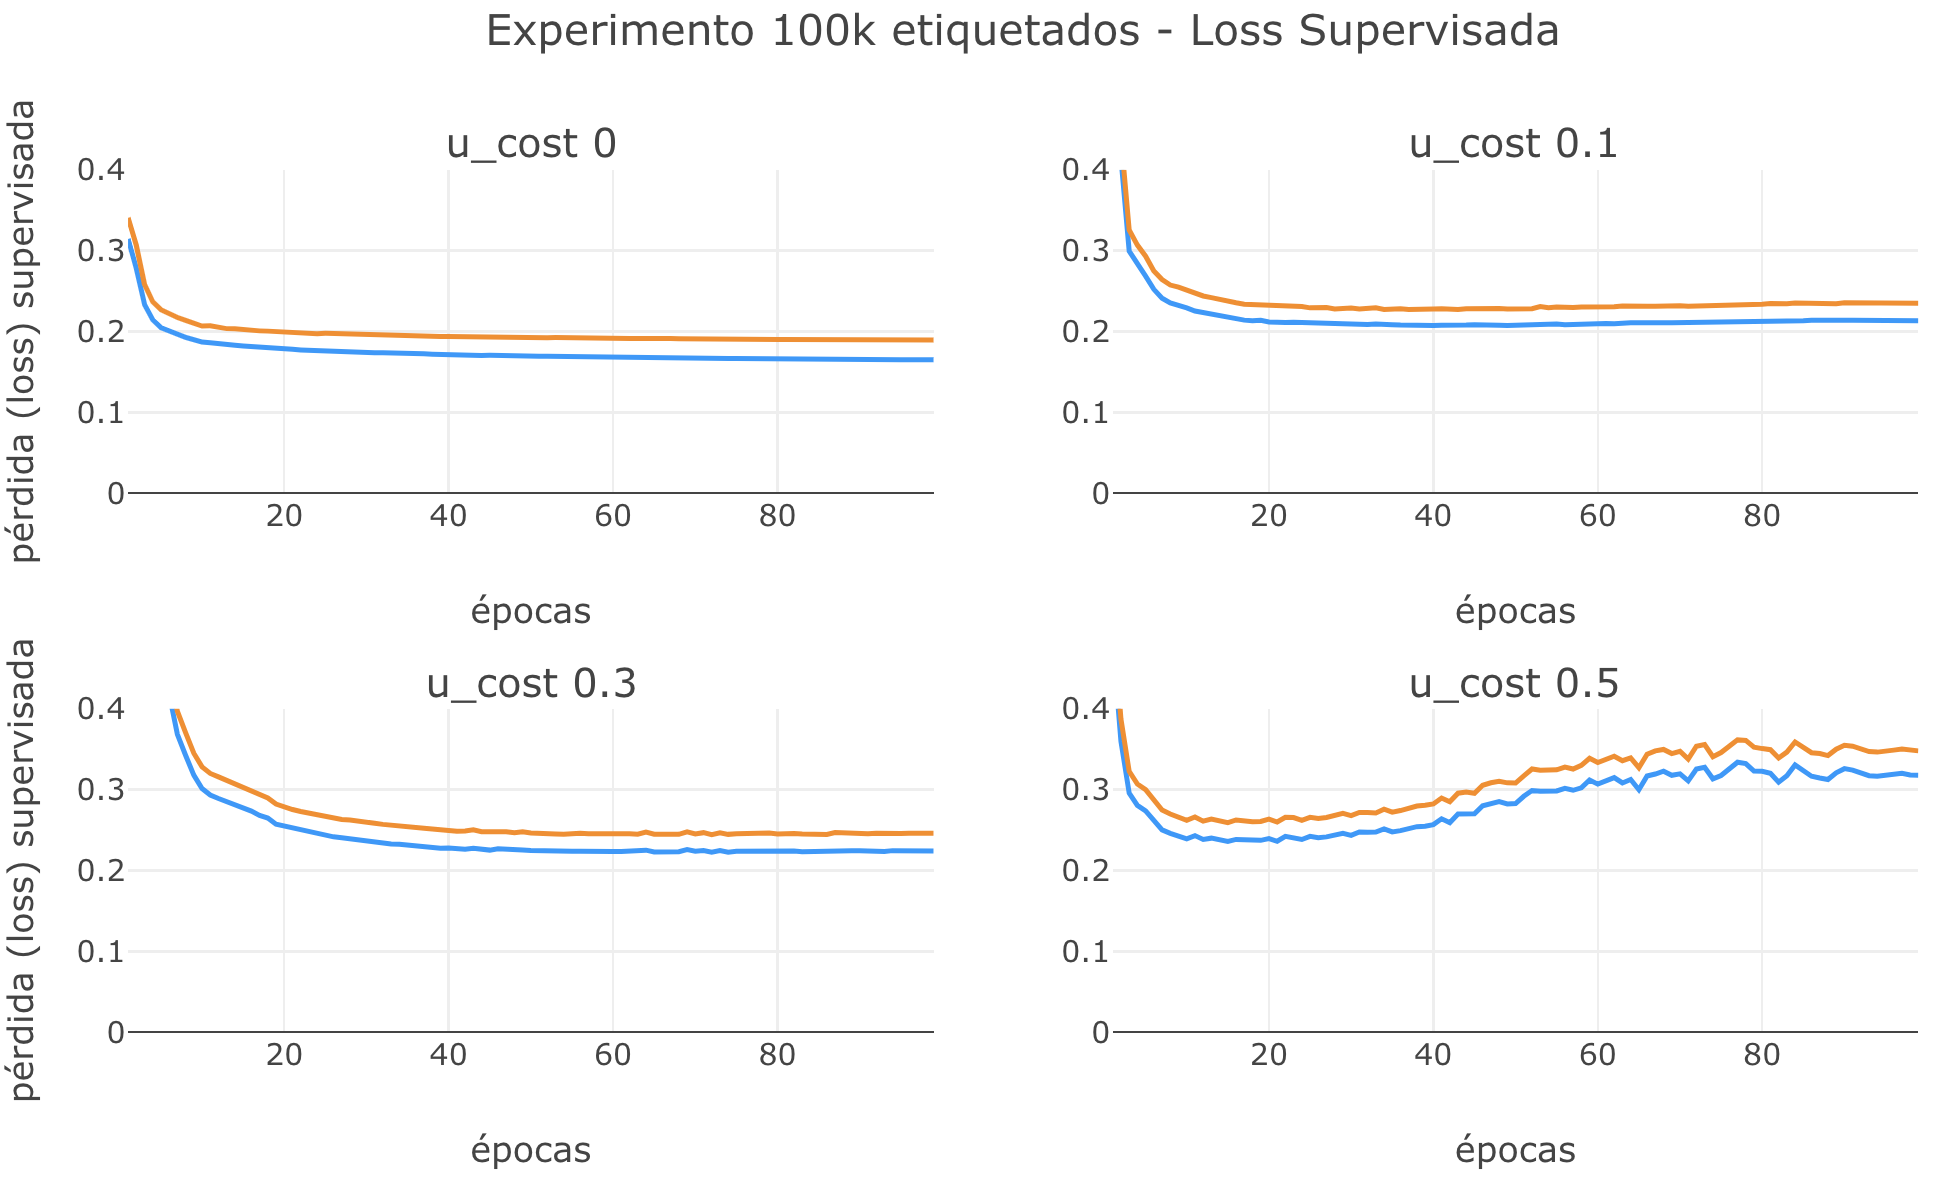
\includegraphics[width=.9\linewidth]{images/CNN_depth_ladder_loss.png}
\caption{Redes convolucionales en escalera experimento CNN-Depth-Ladder-d con variando el factor de la función de costo no supervisado.}
\label{fig:CNN_depth_ladder_loss}
\end{center}
\end{figure}

\subsection{Resultados finales}
% \vspace{5.0mm}

En los Cuadros \ref{table:best_train_CNN_results_table} y \ref{table:best_test_CNN_results_table} se comparan los mejores resultados utilizando la métrica F1-score de los modelos convolucionales. Se observa como los modelos supervisados superan a sus variantes en escalera y que la arquitectura del modelo de redes convolucionales en amplitud performa mejor al modelo de redes convolucionales en profundidad.

\begin{table}[H]
\begin{tabular}{|l|l|l|l|l|l|}
\hline
                    & PER    & LOC    & ORG    & MISC   & O      \\ \hline
CNN wide supervised & \textbf{0.9849} & \textbf{0.9751} & \textbf{0.9775} & \textbf{0.9753} & \textbf{0.9909} \\ \hline
CNN wide ladder     & 0.8152   & 0.8137 & 0.7453  & 0.7194 & 0.9269  \\ \hline
CNN depth supervised & 0.7923 & 0.7847 & 0.6953 & 0.6173 & 0.9837 \\ \hline
CNN depth ladder    & 0.6994 & 0.6628 & 0.4025 & 0.3261 & 0.9732 \\ \hline
\end{tabular}
\caption{F1-score de los mejores modelos por clase sobre los conjuntos de \textbf{entrenamiento} de cada uno de ellos.}
\label{table:best_train_CNN_results_table}
\end{table}


\begin{table}[H]
\begin{tabular}{|l|l|l|l|l|l|}
\hline
                    & PER    & LOC    & ORG    & MISC   & O      \\ \hline
CNN wide supervised & \textbf{0.7341} & 0.7042 & \textbf{0.6039} & \textbf{0.6726} & 0.9325 \\ \hline
CNN wide ladder     & 0.71   & 0.6921 & 0.565  & 0.6317 & 0.906  \\ \hline
CNN depth supervised & 0.7326 & \textbf{0.7089} & 0.5828 & 0.4897 & \textbf{0.9789} \\ \hline
CNN depth ladder    & 0.6876 & 0.6605 & 0.3791 & 0.3099 & 0.9696 \\ \hline
\end{tabular}
\caption{F1-score de los mejores modelos por clase sobre los conjuntos de \textbf{evaluación} de cada uno de ellos.}
\label{table:best_test_CNN_results_table}
\end{table}

Las Figuras \ref{fig:CNN_wide_supervised_ladder_F1-score} y \ref{fig:CNN_depth_supervised_ladder_F1-score} muestran los valores de F1-score para los datos de entrenamiento y evaluación comparando los modelos supervisados y en escalera de los modelos que utilizan las capas convolucionales en amplitud y en profundidad. En ambos casos nuevamente se observa la capacidad de generalización que aporta la tarea no supervisada de los modelos en escalera donde los valores obtenidos sobre el conjunto de evaluación son cercanos al conjunto de entrenamiento.

\begin{figure}[H]
\begin{center}
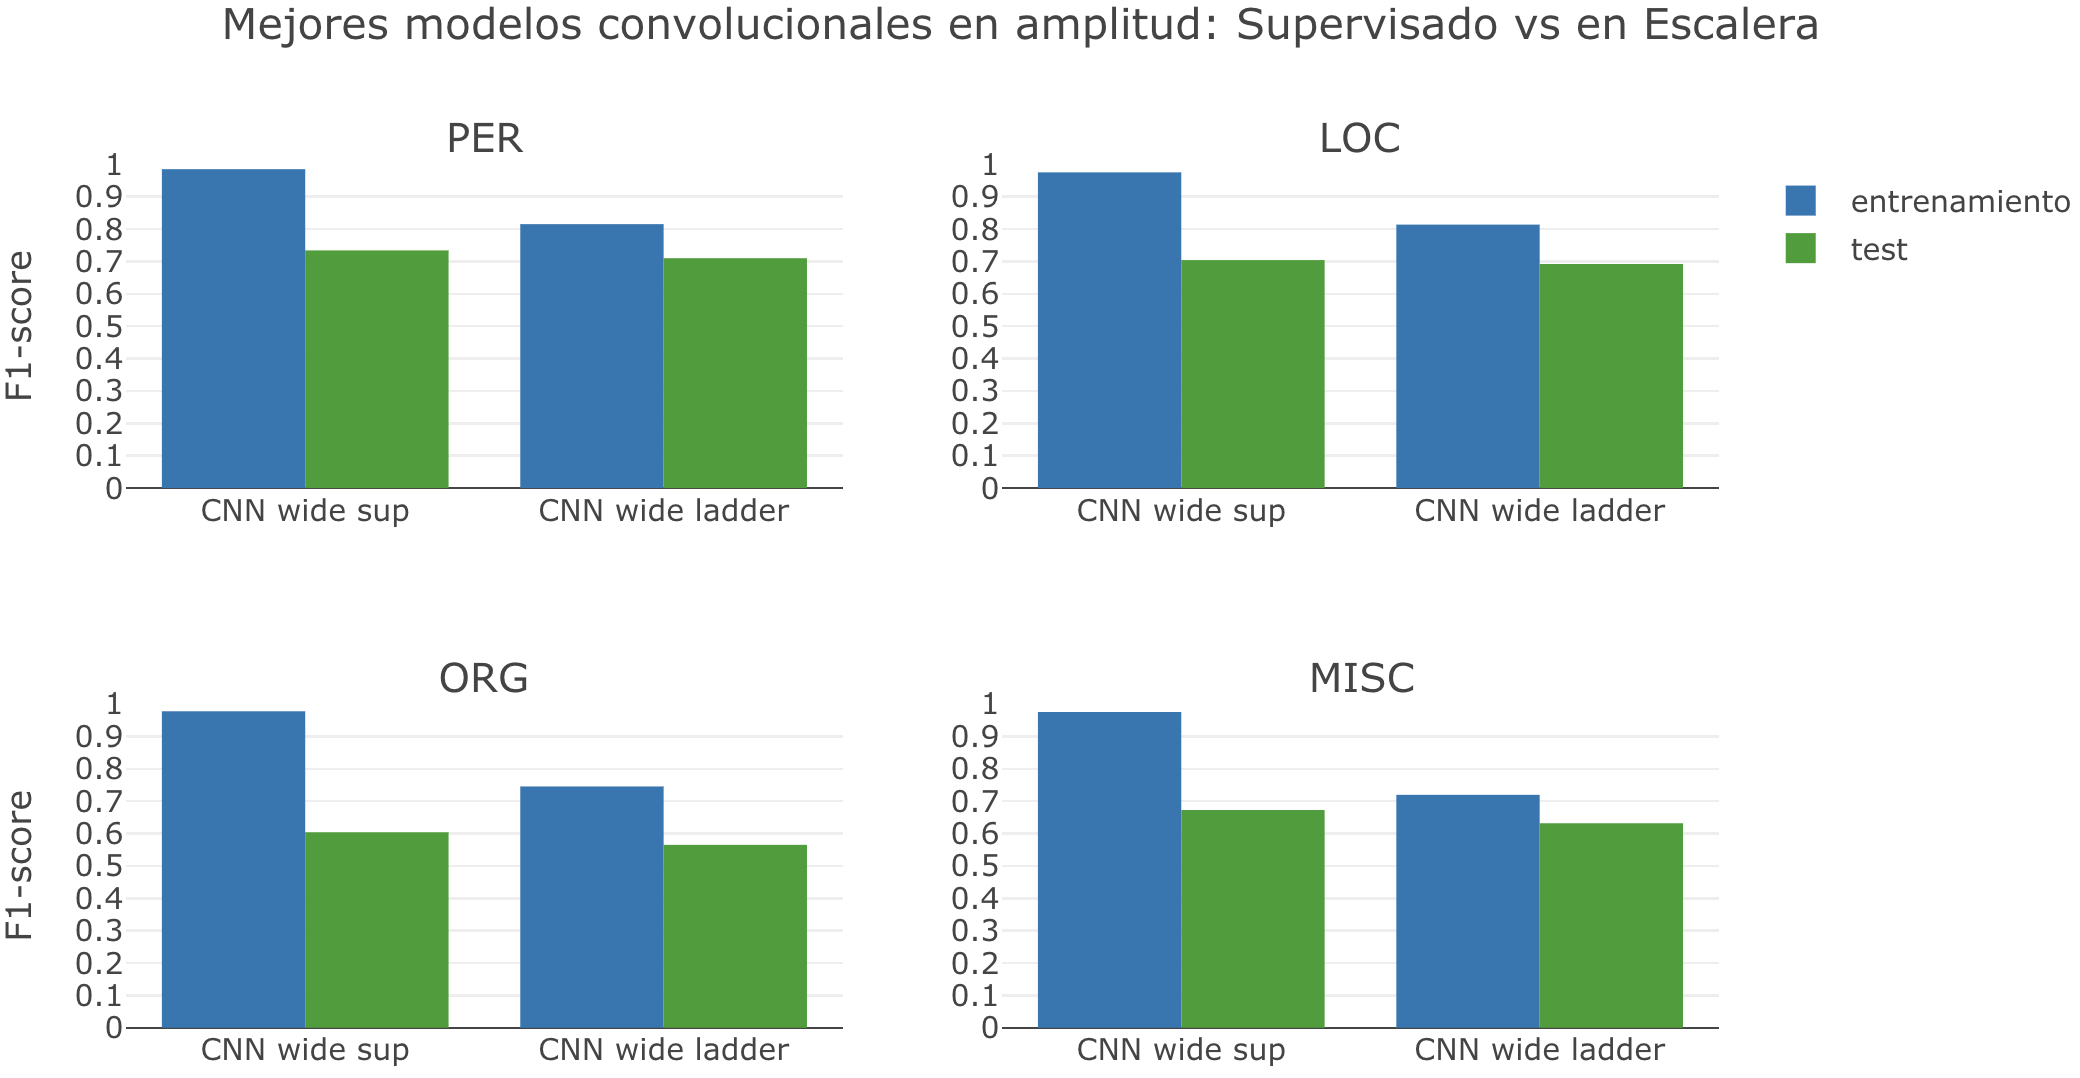
\includegraphics[width=.9\linewidth]{images/CNN_wide_supervised_ladder_F1-score.png}
\caption{}
\label{fig:CNN_wide_supervised_ladder_F1-score}
\end{center}
\end{figure}


\begin{figure}[H]
\begin{center}
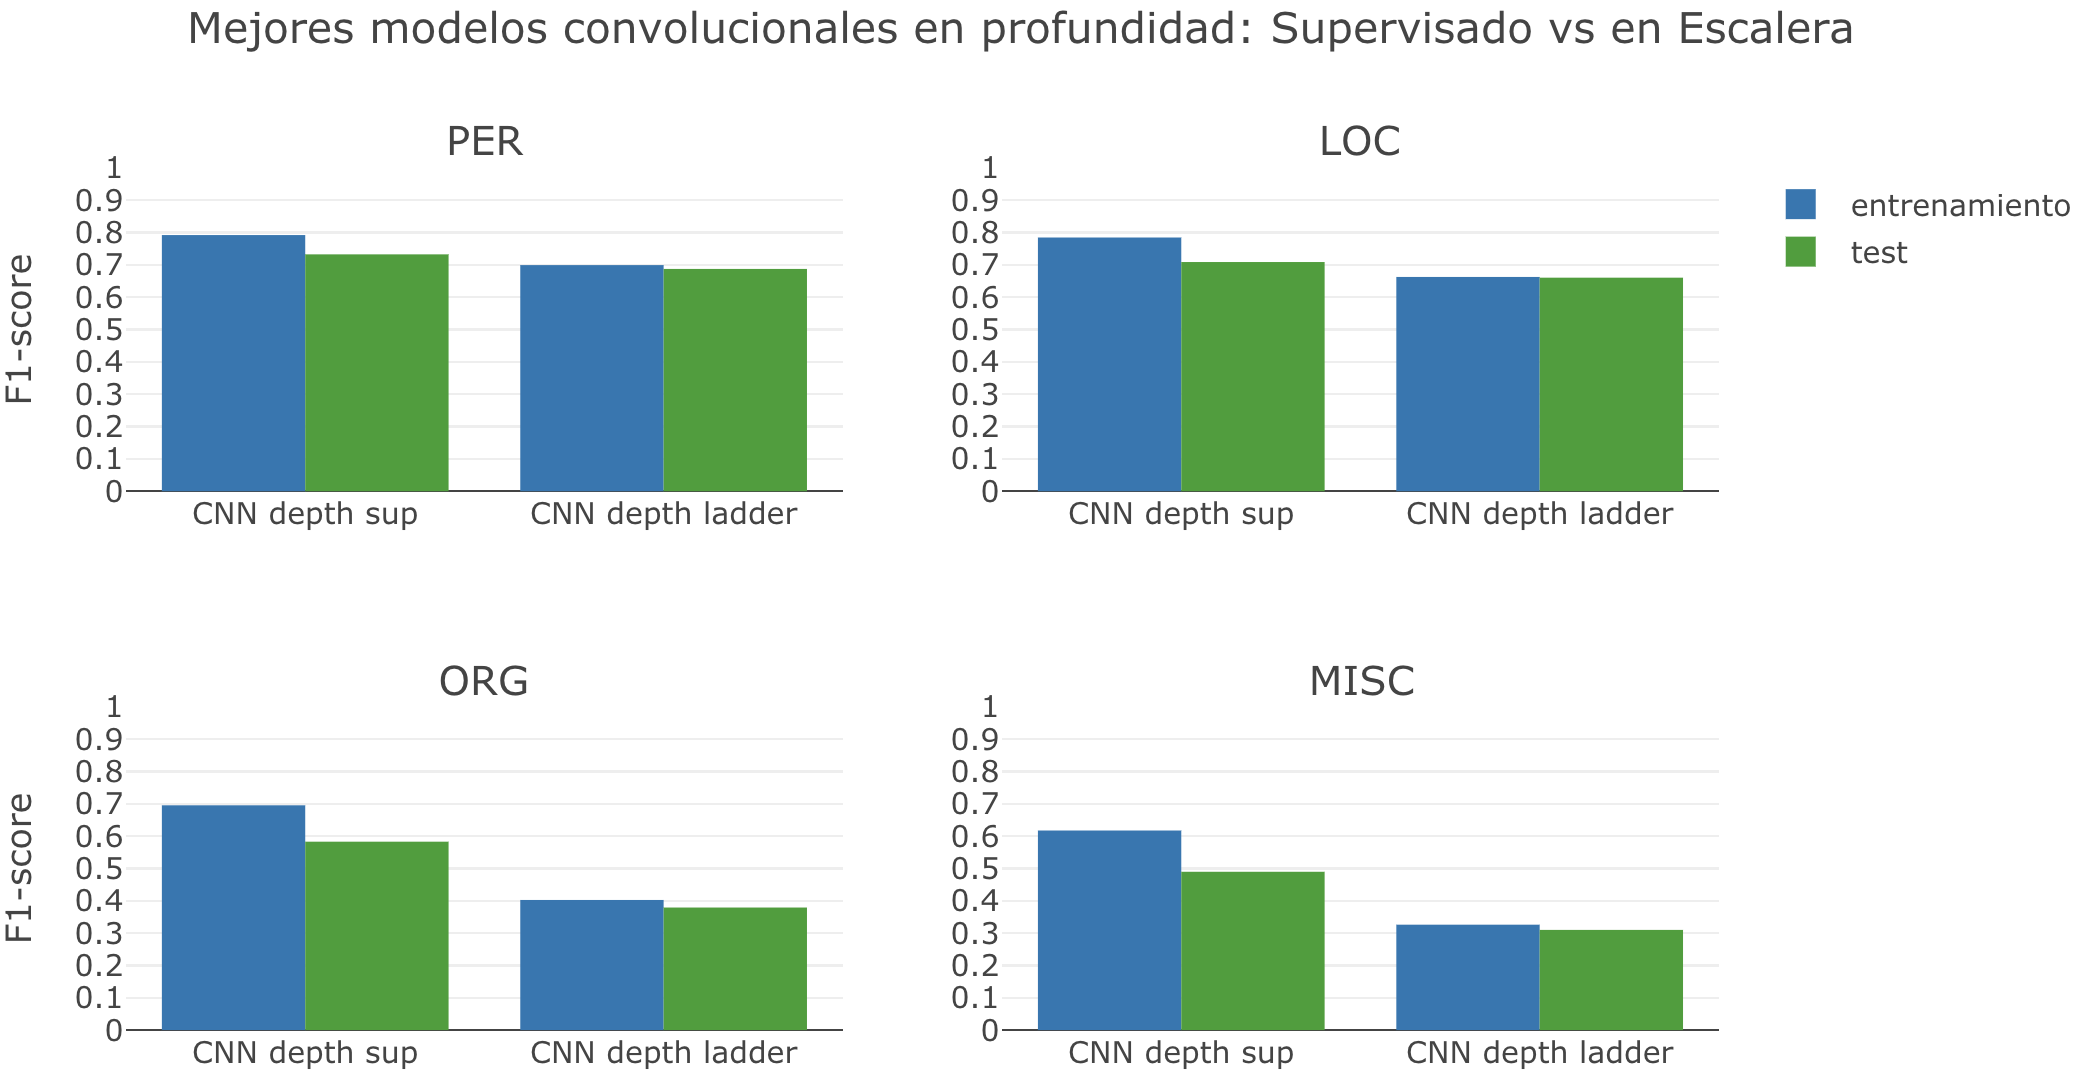
\includegraphics[width=.9\linewidth]{images/CNN_depth_supervised_ladder_F1-score.png}
\caption{}
\label{fig:CNN_depth_supervised_ladder_F1-score}
\end{center}
\end{figure}

\chapter{Conclusiones y trabajo futuro} \label{chapter:chapter5}

\section{Conclusiones}

Una de las primeras problemáticas estudiadas fue la representación vectorial de una palabra dada su semántica en el contexto en el cual ocurre. La estrategia de decaimiento exponencial es la que mejor performa por sobre el resto de estrategias propuestas en el trabajo de \cite{iacobacci-etal-2016-embeddings}. Ponderar en mayor medida a las palabras inmediatamente cercanas a la palabra objetivo tiene sentido, ya que en general aporta mayor información que una palabra distante.

A lo largo del trabajo también se experimentaron modelos basados en redes convolucionales, con el afán de capturar información del contexto de cada palabra al aplicar capas convolucionales. Los resultados determinaron que aplicar convoluciones para extraer características del entorno de una palabra es una alternativa exitosa que supera a la estrategia de decaimiento exponencial.

Al incorporar la tarea no supervisada que proponen las redes neuronales en escalera se observó en distintos experimentos una mayor generalización de estos modelos respecto a los netamente supervisados. Esta mayor generalización puede ser consecuencia de haber compartido las representaciones ocultas de la red entre más de una tarea. 

Agregar una cierta cantidad de datos no anotados al entrenamiento del modelo de redes convolucionales en amplitud en escalera parece ser clave para mejorar el rendimiento del mismo. Sin embargo, se debe tener cuidado de no excederse ya que la red puede no ser lo suficientemente capaz de realizar la tarea no supervisada de reconstrucción de tantos datos no anotados y afectar negativamente al modelo en cuestión. A su vez, es importante regular el peso que se le asigna a la función de costo no supervisada. Si se excede, el modelo diverge ya que se centra demasiado en la tarea de reconstrucción dejando de lado la tarea supervisada de clasificación.

Sobre el modelo de redes convolucionales en profundidad se observó que entrenando el modelo con la totalidad de instancias de entrenamiento y utilizando solo un 25\% se obtienen resultados similares. Vemos entonces la ventaja de trabajar con este modelo semi-supervisado donde tomar una proporción significativamente menor de datos no se corresponde con una gran pérdida de desempeño.

Finalmente, comparando los mejores resultados de cada modelo concluimos los modelos supervisados superan a sus variantes en escalera y que la arquitectura del modelo de redes convolucionales en amplitud tiene mejor desempeño que el modelo de redes convolucionales en profundidad.

\section{Trabajo futuro}

Una metodología interesante para la representación de palabras son los modelos de embeddings de caracteres, en donde el vector representante de una palabra se construye a partir de los \textit{n-grams} de caracteres que la componen. Dado que los caracteres son compartidos entre palabras, estos modelos de \textit{character embeddings} funcionan mejor para representar palabras que están fuera del vocabulario en cuestión. En contraste, modelos de \textit{word embeddings}, como por ejemplo el modelo Word2Vec utilizado en este trabajo de tesis no pueden representar una palabra fuera del vocabulario ya que tratan a cada palabra de forma atómica. Otro aspecto a tener en cuenta es que los modelos de \textit{character embeddings} tienden a generar mejores representaciones para aquellas palabras que aparecen con poca frecuencia, ya que los \textit{n-grams} de caracteres que se comparten entre las palabras aún pueden aprender buenos embeddings. Por otro lado, los modelos de \textit{word embeddings} sufren la falta de oportunidad de entrenamientos suficientes para palabras poco frecuentes.

En el trabajo de \cite{WiNER-Ghaddar-Langlais} se evalúa el desempeño de distintos modelos sobre el conjunto de datos WiNER. En particular, el modelo LSTM-CRF del trabajo de \cite{DBLP:journals/corr/HuangXY15} obtiene los mejores resultados. Este modelo combina el modelo LSTM (Long Short-Term Memory), una red neuronal del tipo recurrente y el método de modelado estadístico CRF (Conditional Random Field). Ambos modelos pertenecen a la familia de modelado de secuencias ya que por su composición les permite lidiar con problemas de series temporales. Surge entonces la idea de combinar las redes convolucionales en escalera estudiadas en este trabajo de tesis con el modelo LSTM-CRF donde el primero se utilizaría para la extracción de features y el segundo encargado de la tarea de clasificación.

Finalmente, como alternativa y en pos de conseguir mejores representaciones de palabras nos gustaría explorar modelos del estado del arte como ELMo (\textit{Embeddings from Language Models}) del trabajo de \cite{DBLP:journals/corr/abs-1802-05365} y BERT (\textit{Bidirectional Encoder Representations from Transformers}) del trabajo de \cite{DBLP:journals/corr/abs-1810-04805}.


\thispagestyle{empty}


%----------------------------------------------------------------------------------------
%	APÉNDICES
%----------------------------------------------------------------------------------------

% \addtocontents{toc}{\vspace{2em}} % Agrega espacios en la toc

% \appendix % Los siguientes capítulos son apéndices

%  Incluye los apéndices en el folder de apéndices

% \include{Apendices/Ap}
\thispagestyle{empty}
%\include{Apendices/AppendixB}
%\include{Apendices/AppendixC}

\addtocontents{toc}{\vspace{2em}} % Agrega espacio en la toc


%----------------------------------------------------------------------------------------
%	BIBLIOGRAFÍA
%----------------------------------------------------------------------------------------
\backmatter
\nocite{*}
\bibliographystyle{apalike}
\bibliography{bibliografia.bib} 
%Aquí ponen el nombre del archivo .bib

\end{document}